% ********** Theory Chapter **********
\chapter{The Theory of  Cold-Electron Bolometers}
\label{cha:theory}
\epigraph{`An experiment is a question which science poses to Nature, and a measurement is the recording of Nature's answer.'}{\mbox{\textup{---\textsc{Max Planck}}}}
%
\section{Introduction}\label{sec:theory-introduction}
As with all areas of study within physics, the fabrication and testing of cold-electron bolometers draws together elements from several fields. These include electronics, concepts from quantum mechanics (such as electron tunnelling), cryogenics, and low temperature physics, as well as solid-state physics. The study and testing of a cold-electron bolometer requires a strong understanding of these areas, as well as a general grounding in the field of instrumentation and its associated vocabulary. Furthermore, it is important to arrive at a model that might be used not only to describe the observed behaviour of the devices being studied but may, when applied with common sense, be used to extrapolate the performance of a device in various scenarios. The following chapter describes the physics which underlies cold-electron bolometer and then details how this is applied to arrive at models which describe the performance of such a detector. Particular note is given to the phenomena which limit the sensitivity of a detector and how such sensitivity might be quantified.
%
\section{Tunnelling Barriers}\label{sec:tunnelling-barreirs}
As will be explained in the following sections, the cold-electron bolometer directly removes hot electrons from the detector's absorber. This thermally selective removal of charges is made possible through the use of a tunnelling barrier. This tunnelling barrier allows the electron systems on either side to be separated (i.e. the energy levels in the two do not have to be aligned). 
\par 
Several types of tunnelling barriers exist, however only those involving a superconductor shall be considered here, since this is a requirement of the thermal selection required for a cold-electron bolometer. The four main types of contact used in cold-electron bolometers are:
\begin{description}
\item[Normal metal-Insulator-Superconductor (\glstext{acr:NIS})] The simplest (at least conceptually); the two sides (the normal metal and the superconductor) are separated by an insulating layer (typically an oxide layer).
\item[Superconductor-Insulator-Superconductor (\glstext{acr:SIS})] This is essentially the same as the arrangement described above, except that the normal metal is replaced by the same material as is used on the other side of the barrier.
\item[Superconductor-Insulator-(different) Superconductor (\glstext{acr:SIS2})] A further progression of the systems already described; here the materials on either side of the insulator are both superconductors but have different energy gaps (they are different superconductors).
\item[Semiconductor-Superconductor (\glstext{acr:SmS})] This structure replaces the insulator with a Schottky barrier, which forms naturally between the semiconductor and a metal (or superconductor). Typically (and for all the work described in this thesis), a highly doped semiconductor, which can be thought of as being metallic (since there is no discernible band gap), is used.
\end{description}

\subsection{Formation of Insulating Layers}
\label{ssec:tunnelling-barreirs-formation}
From the above list, it can be seen that only two types of insulating barriers are typically used in the fabrication of cold-electron bolometers. These are: oxide layers and Schottky barriers. While both of these can be thought of as performing the same function, their formation is very different. An oxide layer requires an additional stage during the device fabrication process, where oxygen is introduced to the evacuated deposition chamber. A Schottky barrier, on the other hand, will form naturally between a semiconductor and a metal (or superconductor); this means that no additional fabrication stages are required.
\par 
An oxide insulating layer forms  ionic bonds between the atoms of the metal and the oxygen atoms. This prevents the outer electrons in the metal, which previously were \textit{free} and available for current flow, from being able to flow as current and thus the resistance of the material is greatly increased.
\begin{figure}[t]
\begin{center}
\subfloat[]{
	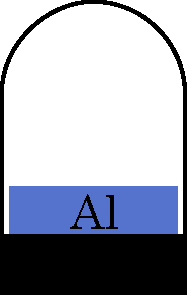
\includegraphics[width=0.15\textwidth]{figures/Oxide_Growth_AlDep}
	\label{fig:OxideGrowth_AlDep}
}
\hspace{0.2\textwidth}
\subfloat[]{
	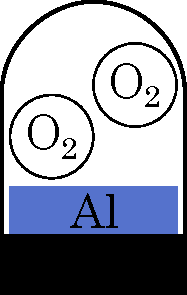
\includegraphics[width=0.15\textwidth]{figures/Oxide_Growth_O2intro}
	\label{fig:OxideGrowth_O2intro}
}
\hspace{0.2\textwidth}
\subfloat[]{
	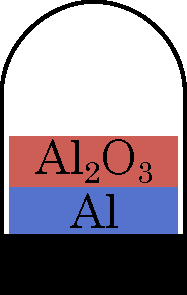
\includegraphics[width=0.15\textwidth]{figures/Oxide_Growth_final}
	\label{fig:OxideGrowth_final}
}
\\
\subfloat[]{
	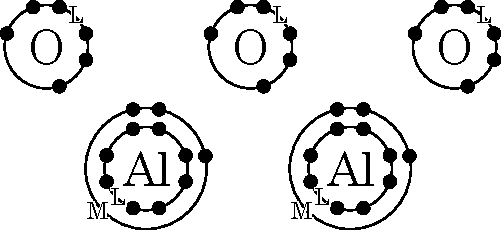
\includegraphics[width=0.4\textwidth]{figures/Al2O3_formation_start}
	\label{fig:AlOxideFormation_start}
}
\hspace{0.1\textwidth}
\subfloat[]{
	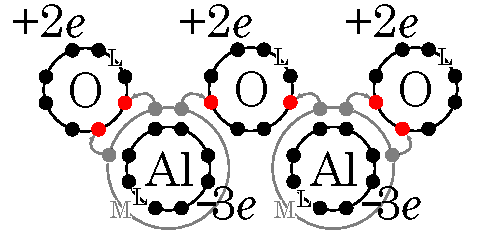
\includegraphics[width=0.4\textwidth]{figures/Al2O3_formation_end}
	\label{fig:AlOxideFormation_end}
}
\caption[Growth and chemical fabrication of a metal-oxide layer]{Growth (a)--(c) and ionic bond formation (d) and (e) of an aluminium oxide (Al\textsubscript{2}O\textsubscript{3}) layer. (a) Aluminium has been deposited (usually via evaporation) in a vacuum. (b) Oxygen is introduced into the evaporation chamber. (c) The oxygen atoms form ionic bonds with the aluminium, this causes the growth of an aluminium oxide layer at the surface of the deposited aluminium. (d) Oxygen and aluminium atoms prior to bonding; oxygen contains six electrons in the L electron shell (1s\textsuperscript{2} 2s\textsuperscript{2} 2p\textsuperscript{4}), aluminium contains a full L electron shell and has three electrons in its M shell (1s\textsuperscript{2} 2s\textsuperscript{2} 2p\textsuperscript{6} 3s\textsuperscript{2} 3p\textsuperscript{1}). (e) The electrons from the M shells in the aluminium atoms (shown in grey for clarity) move to the L shell  of the oxygen atoms (shown as the red electrons); this is the formation of ionic bonds and results in both the oxygen and aluminium atoms having their L shells filled (for tidiness, the full K shell is not shown).}\label{fig:AluminiumOxideGrowth}
\end{center}
\end{figure}
\par 
The formation of an oxide layer is conceptually simple. Since aluminium is commonly used \parencite[for example those described by][]{Clark2005, Pekola2004, Prest2011} as one side of a tunnelling contact, aluminium oxide often forms the insulating oxide. Figure~\ref{fig:AluminiumOxideGrowth} and the following explain the growth of an aluminium-oxide layer, however, other oxide layers are sometimes used in similar devices, for example the tantalum oxide based devices described by \textcite{Chaudhuri2014}. After the metal has been deposited, by evaporation or other means (Figure~\ref{fig:OxideGrowth_AlDep}), oxygen is introduced into the deposition chamber (Figure~\ref{fig:OxideGrowth_O2intro}). The outermost electrons from the aluminium (those in the third shell, the M shell) move to the vacant states in the outer shell of the oxygen atoms (oxygen has two vacant electron states in its second shell, the L shell), forming ionic bonds between the aluminium and the oxygen; this is shown in Figures~\ref{fig:AlOxideFormation_start} and \ref{fig:AlOxideFormation_end}. This results in a layer of aluminium oxide (Al\textsubscript{2}O\textsubscript{3}) forming on top of the deposited aluminium (Figure~\ref{fig:OxideGrowth_final}).
\par 
While conceptually simple, in order to produce an even, high quality layer of a desired thickness, great care needs to be taken regarding both the quantity of gas introduced and the temperature of the chamber during the introduction of the oxygen gas \citep{Cabrera1949, Jaeger1991}. The addition of an oxide layer also necessitates an additional step in the fabrication, along with the required equipment to add and monitor the flow of gas into the deposition chamber.
\par 
As opposed to an oxide layer, a Schottky barrier will form naturally between a metal and a semiconductor. The barrier is formed as the electrons in the two materials move to cause the Fermi-energy in the two materials to be aligned. The concept of a naturally forming potential barrier between a semiconductor and a metal was first suggested by \textcite{Schottky1939} whose original explanation is illustrated in Figure~\ref{fig:SchottkyFormation}
\begin{figure}[t]
\begin{center}
\subfloat[]{
	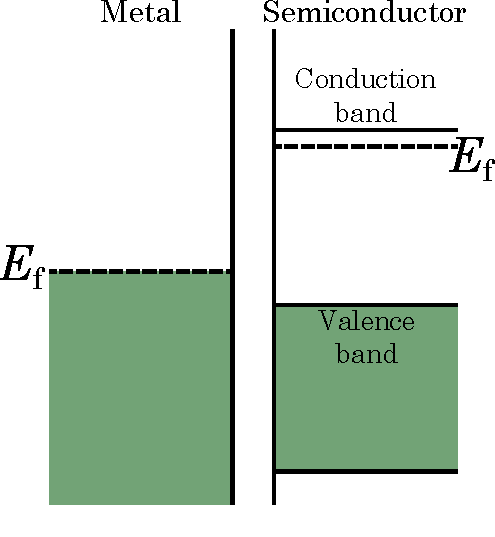
\includegraphics[width=0.30\textwidth]{figures/SchottkyFormation_before}
	\label{fig:SchottkyFormation_before}
}
%\hspace{0.125\textwidth}
\subfloat[]{
	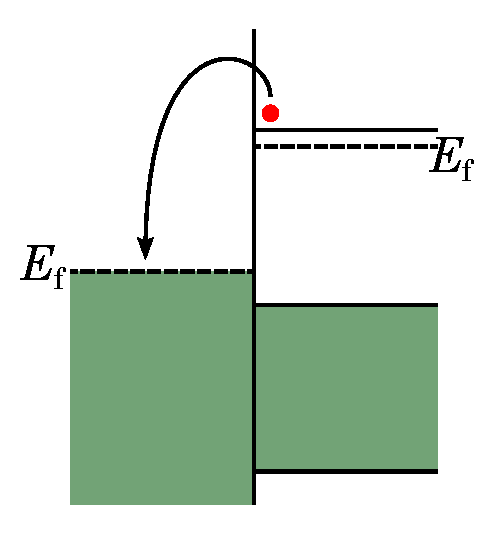
\includegraphics[width=0.30\textwidth]{figures/SchottkyFormation_after}
	\label{fig:SchottkyFormation_after}
}
%\hspace{0.125\textwidth}
\subfloat[]{
	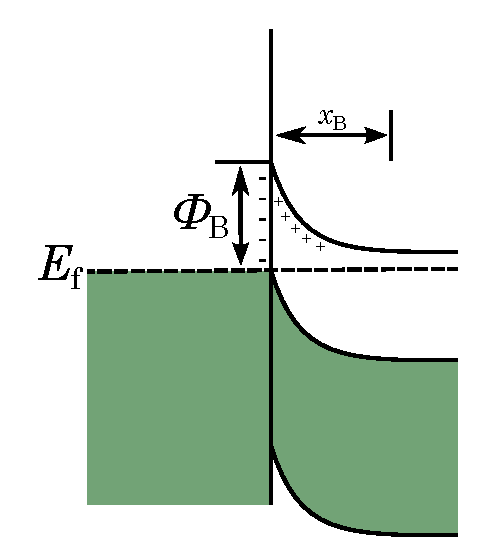
\includegraphics[width=0.30\textwidth]
	{figures/SchottkyFormation_equilibrium}
	\label{fig:SchottkyFormation_equilibrium}
}
\caption[Formation of a Schottky barrier]{Formation of a Schottky barrier between a metal and an n-doped semiconductor. (a) Before being brought into contact, the energy distribution in the metal and the semiconductor are independent, with the Fermi-level ($E_{\mathrm{f}}$, shown as the dashed line) sitting at the top of the occupied states in the metal (shown at $T = 0~\mathrm{K}$) and just below the conduction band of the semiconductor. (b) Immediately after the metal and semiconductor are brought into contact, the energy levels are unchanged; however, electrons (red circle) start to move from the conduction band of the semiconductor to the vacant lower energy states in the metal. These electrons leave behind positively charged ions or \textit{donor states}. (c) The movement of the most energetic electrons from the semiconductor causes the Fermi-level to move, this continues until the Fermi-level in both the materials is the same. Away from the interface, the band structure of the semiconductor moves relative to the Fermi-level; at the interface, however, this is not the case, which causes the phenomenon know as \textit{band-bending} in the semiconductor. The height of the Schottky barrier established is related to the difference between the vacuum level in the two materials and is given by $\varPhi_{\mathrm{B}}$.} \label{fig:SchottkyFormation}
\end{center}
\end{figure}
\par
Schottky's explanation was that, after the semiconductor has been brought into contact with the normal metal, the electrons in the conduction band of the semiconductor (the most energetic) are able to move to the lower (energetically favourable) states above the Fermi-level in the metal (illustrated in Figure~\ref{fig:SchottkyFormation_after}), leaving behind positively charged \textit{donor} ions. This causes the Fermi level within the semiconductor to decrease, since there are fewer electrons in the conduction band. This movement of electrons continues until there is an equilibrium established between the electron systems in the two materials (i.e. when the Fermi levels are aligned). Away from the interface between the metal and the semiconductor, the valence and conduction bands move relative to the Fermi level; however, at the interface, the bands move differently, since it is these electrons which have moved. This causes the phenomenon of \textit{band-bending} and the formation of a depletion region (from $E_{\mathrm{f}}$ to $E_{\mathrm{f}} + \varPhi_{\mathrm{B}}$) in the semiconductor at the interface.
\par
Schottky barriers between doped silicon and aluminium typically have a height of $\varPhi_{\mathrm{B}} = 0.7~\mathrm{eV}$ \parencite{Yu1970}. \textcite{Archer1970} show that increasing the doping of the silicon to very high levels (on the order of say $N_{\mathrm{D}} = 10^{19}~\mathrm{cm^{-3}}$), as is the case in the materials used in this work, lowers the barrier height by a factor of up to $1.5$ from the undoped level (which remains constant up to doping concentrations of $\sim 10^{16}~\mathrm{cm^{-3}}$). In either case this value is still substantially large than the energy gap of the superconducting aluminium, which has a nominal value of $2\varDelta = 364~\mathrm{\upmu eV}$ at $0~\mathrm{K}$.
\par 
The width of the barrier, $x_{\mathrm{B}}$, on the other hand depends heavily on the level of doping in the semiconductor. As shown in Figure~\ref{fig:SchottkyFormation} the formation of a Schottky barrier requires enough electrons to move from the semiconductor to the metal to bring the Fermi levels into alignment. In a lightly-doped semiconductor, where free electrons are sparse, electrons must move from further into the semiconductor to achieve this, resulting in a wider barrier compared to the highly-doped case where sufficient electrons can be found close to the interface. \textcite{Kittel2005} provides a rough approximation of the barrier width to be:
\begin{align}
x_{\mathrm{B}} = 	
	\sqrt{\frac{2\varepsilon\varepsilon_{0}\left|\varPhi_{\mathrm{B}}\right|}
	{N_{\mathrm{D}}e}}\,, \label{eqn:barrierWidth}
\end{align}
where $\varepsilon$ and $\varepsilon_{0}$ are the relative and vacuum permittivity. Using typical values for the materials studied in this work of $\varepsilon = 11.68$ and $N_{\mathrm{D}} = 4 \times 10^{19}~\mathrm{cm^{-3}}$, along with the value of $\varPhi_{\mathrm{B}} = 0.7~\mathrm{eV}$ from above, yields a barrier width of $x_{\mathrm{B}} = 4.7~\mathrm{nm}$ in this case. Simplistically the barrier width changes as:
\begin{align}
x_{\mathrm{B}} \propto \sqrt{\frac{1}{N_{\mathrm{D}}}}\,. 
\label{eqn:barrierWdithApprox} 
\end{align}
\par  
Schottky barriers are, in theory, simple to fabricate. All that is required is for the two materials to be deposited sequentially. An important caveat is that one must ensure that the first material deposited (often the semiconductor) is free of impurities or unwanted surface films (such as oxide layers). This is simple if the entire fabrication process can be performed in a single system under continuous vacuum. If, however, the device needs to be removed from the protection of the evacuated deposition system (to be patterned, for example), then it is important to ensure that the surface is thoroughly cleaned prior to the deposition of the second material \parencite[a good description of surface preparation requirements is given by][]{Roccaforte2003}. Should the surface of the first material not be sufficiently cleaned, contamination may either cause an insulating layer to form which, while itself acting as a tunnelling barrier, will inhibit or stop the development of a Schottky barrier; or alter the Fermi-level of the material and thus alter the Schottky barrier height (as discussed in the following paragraph).
\par 
One cannot simply choose any combination of semiconductor and metal to create a Schottky barrier. As can be seen from the description above and Figure~\ref{fig:SchottkyFormation}, there needs to be a difference between the inherent Fermi-levels in the two materials. If this is not the case, when the two materials are brought together, there will be minimal movement of electrons from the semiconductor's conduction band to the metal. This will cause the barrier height, $\varPhi_{\mathrm{B}}$, to be very small. A similar effect is observed when the Fermi level of the metal is higher than that of the semiconductor; this results in the band-bending, seen in Figure~\ref{fig:SchottkyFormation_equilibrium}, to be downwards. This means that electrons do not encounter a barrier. Contacts of this type are known as \textit{ohmic contacts}. A more detailed description of the formation and criteria for ohmic contacts is given by \textcite{Rhoderick1988} who also offer an excellent overview on the concepts relating to Schottky barriers.

\section{The Tunnelling Current}\label{sec:theory-current}
\begin{figure}[t]
\begin{center}
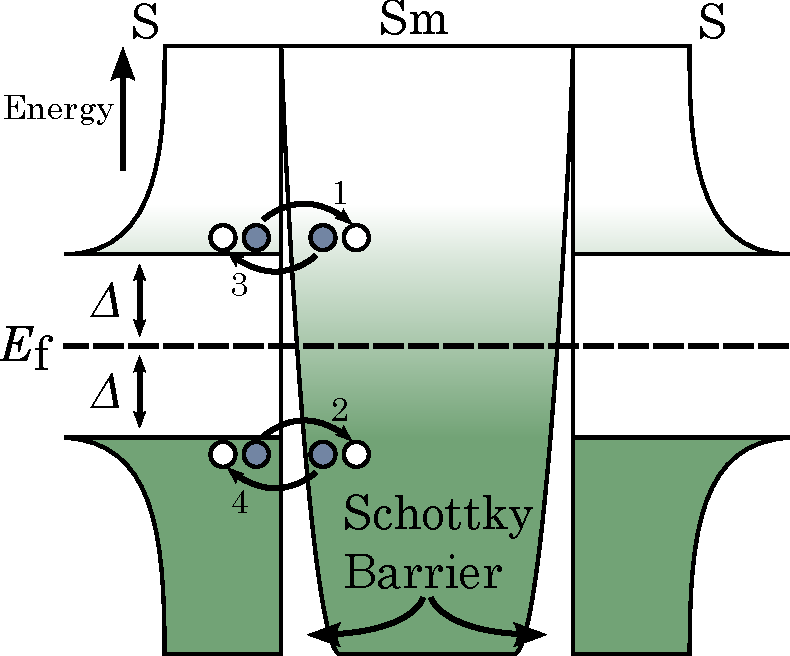
\includegraphics[height = 0.5\textheight]{figures/CEB_energyLevels_noBias}
\caption[Possible tunnelling of charges in a SiCEB]{Possible tunnelling of charges in a \gls{acr:SSmS} structure, shown at non-zero temperature,  without any external bias across this system and for only one junction. The density of the shading represents the number of occupied states. Numbering as listed on Page~\pageref{list:tunnellingOptions}.}
\label{fig:IVmod:energyLevels-noBias}
\end{center}
\end{figure}
In order to understand the behaviour of a cold-electron bolometer, it is important to understand the movement of charges, at different energies, across the tunnelling barrier. To do this, we need to consider four directions of charge transfer, these are\footnote{In the following list $E_{\mathrm{f_{S}}}$ is used to denote the Fermi energy in the superconductor.}:
\begin{enumerate}\label{list:tunnellingOptions}
	\item Charges in the superconductor with energies above the superconducting 
			bandgap $\left(E > E_{\mathrm{f_{S}}} + \varDelta\right)$ tunnelling into the 
			central semiconductor island.
	\item Quasiparticles in the 
			superconductor whose energies are below the Fermi-energy 
			$\left(E < E_{\mathrm{f_{S}}} - \varDelta\right)$ tunnelling into the 
			central island. 
	\item Charges in the central island, with energy levels corresponding to the 
			normal states in the superconductor 
			$\left(E > E_{\mathrm{f_{S}}} + \varDelta\right)$, tunnelling into these states.
	\item Charges in the central island, with energies corresponding to below the
			superconducting states in the superconductor 
			$\left(E < E_{\mathrm{f_{S}}} - \varDelta\right)$, tunnelling into these states.
\end{enumerate}
Since the movement of charges in terms 3 and 4 is the opposite of those in the first two terms, these act to suppress the total current.
\par
Figure~\ref{fig:IVmod:energyLevels-noBias} shows these four possible forms of tunnelling when there is no bias across the structure. It can be seen that the tunnelling routes represented by numbers 1 and 3 are possible (providing there is sufficient thermal broadening of the density of states), since there are charges and vacant states on both sides of the Schottky barrier. The tunnelling shown by numbers 2 and 4 are less likely, since there are very few vacant states for electrons to tunnel to.
\begin{figure}[t]
\begin{center}
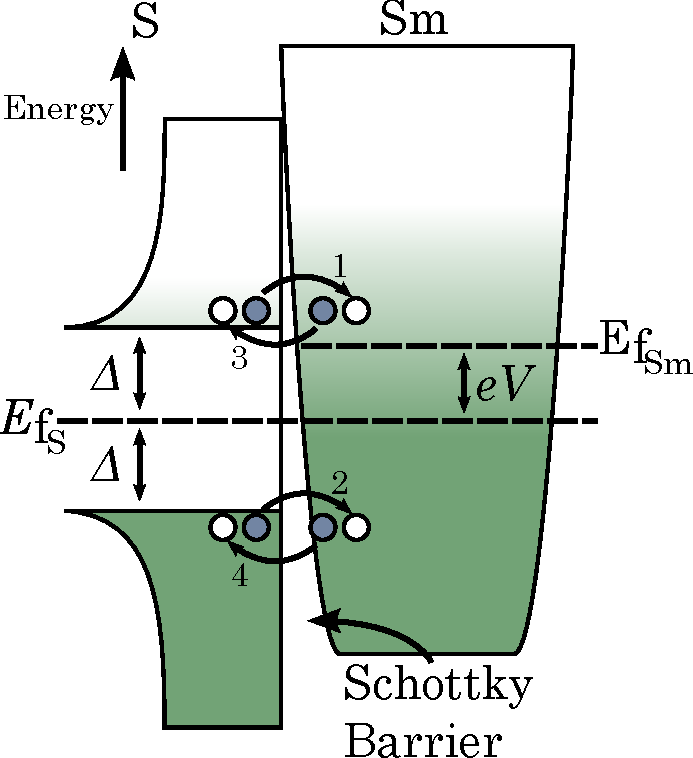
\includegraphics[height = 0.5\textheight]{figures/CEB_energyLevels_+veBias}
\caption[Tunnelling in of charges across a positively biased device]{Tunnelling of charges across a single superconductor-semiconductor junction when biased by a voltage, $V$, such that the Fermi level in the semiconductor, $E_{\mathrm{f_{Sm}}}$, is raised above that of the superconductor, $E_\mathrm{{f_{S}}}$.}
\label{fig:IVmod:energyLevels-+Bias}
\end{center}
\end{figure}
\par
By applying an external bias across the structure, it is possible to shift the distribution of charges in the three layers relative to each other. This biasing causes the probability of tunnelling via each of the routes to be altered. Figure~\ref{fig:IVmod:energyLevels-+Bias} shows the effect of biasing a single junction structure such that the energy levels in the semiconductor (right) are raised above the energy levels in the superconductor (left). This has a notable effect to the probability of tunnelling via each of the described routes. Charges are less likely to tunnel from the superconductor into the semiconductor (routes one and two), since there are fewer states available in the semiconductor. Conversely, charges are more likely to move from the semiconductor into the superconductor (routes three and four) as there are a greater number of occupied states in the semiconductor with energies corresponding to the vacant states in the superconductor.
\begin{figure}[t]
\begin{center}
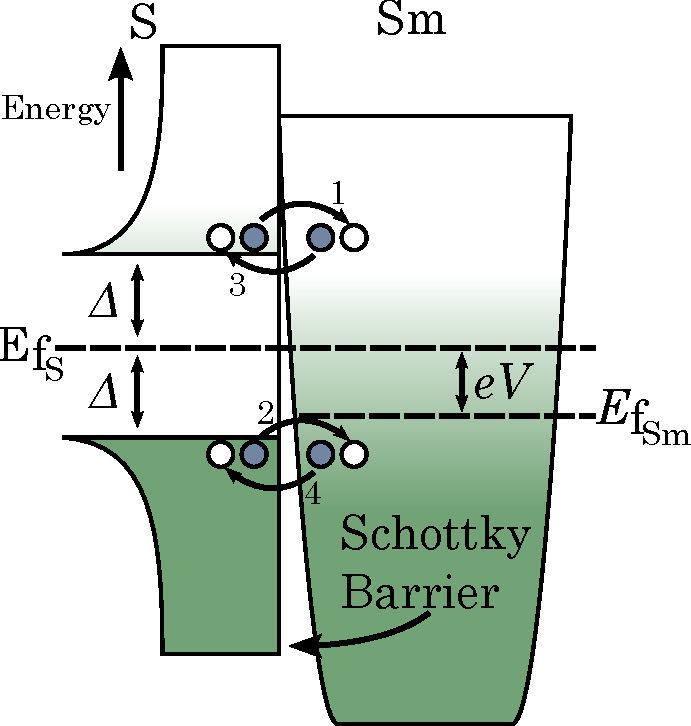
\includegraphics[height = 0.5\textheight]{figures/CEB_energyLevels_-veBias}
\caption[Tunnelling in of charges across a negatively biased device]{Tunnelling of charges across a single superconductor-semiconductor junction when biased in the opposite polarity to that shown in Figure~\ref{fig:IVmod:energyLevels-+Bias}. The biasing voltage, $V$, causes the Fermi level in the superconductor, $E_{\mathrm{f_{S}}}$, to be raised above the Fermi level in the semiconductor, $E_{\mathrm{f_{Sm}}}$.}
\label{fig:IVmod:energyLevels--Bias}
\end{center}
\end{figure}
\par 
Figure~\ref{fig:IVmod:energyLevels--Bias} illustrates a single junction system biased in the opposite polarity to the structure shown in Figure~\ref{fig:IVmod:energyLevels-+Bias}. In this case, when compared to the unbiased state, charges are more likely to tunnel from the superconductor into the semiconductor (routes one and two), since the occupied states in the superconductor correspond to a greater number of vacant states in the semiconductor. Likewise, fewer charges will tunnel from the semiconductor into the superconductor (routes three and four), as there are fewer occupied states in the semiconductor aligned with vacant states in the superconductor.
\par 
When modelling the current in a two junction system, it is useful to note that, since the two junctions can be thought of as resistors in series, we need only consider the current through one junction, since the current through each of the junctions will be the same. This leads to two important definitions in the following derivation: the voltage used in these equations is defined to be the voltage dropped across a two junction system. The following equations assume that there is no resistance to current flow from either the semiconductor or superconductor, hence the voltage dropped across each junction will be $\nicefrac{V}{2}$. The second definition to note is that the tunnelling resistance, $R_{\mathrm{N}}$, is defined to be the resistance of a single junction.
\par
For each of these movements of charge, it is possible to define a Fermi distribution, $q_{\mathrm{n}}$, where the subscript $\mathrm{n}$ corresponds to the number of the term in the list on Page~\pageref{list:tunnellingOptions}.
\begin{align}
q_{1} &\sim \frac{1}{\e^{\frac{\left|E\right|}{k_{\mathrm{B}}T_{\mathrm{S}}}}+1}\,, \\
q_{2} &\sim \frac{1}{\e^{\frac{-\left|E\right|}{k_{\mathrm{B}}T_{\mathrm{S}}}}+1}\,, \\
q_{3} &\sim \frac{1}{\e^{\frac{\left(\left|E\right|+
				\nicefrac{eV}{2}\right)}{k_{\mathrm{B}}T_{\mathrm{e}}}}+1}\,, \\
q_{4} &\sim \frac{1}{\e^{\frac{-\left(\left|E\right|- 
					\nicefrac{eV}{2}\right)}{k_{\mathrm{B}}T_{\mathrm{e}}}}+1}\,. 
\end{align}
\par
In these equations, $E$ is the energy of a carrier, $k_{\mathrm{B}}$ is Boltzmann's constant, $T_{\mathrm{S}}$ and $T_{\mathrm{e}}$ are the temperatures of the charge carries in the superconductor and the central island respectively, $e$ is the electron charge and $V$ is the voltage across the structure. $q_{1}$ is the Fermi-distribution for charges in the superconductor with energy above the superconducting bandgap, $q_{2}$ relates to charges in the superconductor with energies below the bandgap, $q_{3}$ and $q_{4}$ are the distributions of charges in the central island with energies above and below the superconductor's bandgap respectively.
\par 
For each of the terms in the above list, we can define a probability $p_{1\mbox{--}4}$ that a charge will tunnel in the stated manner. This probability is related to the likelihood of an occupied state on one side of the tunnelling barrier corresponding to an empty state on the other side. For each of the forms of tunnelling defined above, this probability is:
\begin{align}
p_{1} &= q_{1} \times \left(1 - q_{3}\right)\,, \label{eqn:IVmodp1}\\
p_{2} &= q_{2} \times \left(1 - q_{4}\right)\,, \label{eqn:IVmodp2}\\
p_{3} &= q_{3} \times \left(1 - q_{1}\right)\,, \label{eqn:IVmodp3}\\
p_{4} &= q_{4} \times \left(1 - q_{2}\right)\,. \label{eqn:IVmodp4}
\end{align}
\par 
The total movement of charges between the superconductor and the superconducting contact is related to the sum of these probabilities integrated over all energies and, if movement from the superconductor to the semiconductor is taken to be the positive direction, is given by:
\begin{align}
p_{_{\mathrm{T}}} &= \int_{0}^{\infty} \left[ p_{1} + p_{2} - p_{3} - p_{4} \right]
				\mathrm{d}E \,. \label{eqn:IVmod_Pt_start}
\end{align}
Substituting the terms for $p_{1-4}$ from Equations~\ref{eqn:IVmodp1}--\ref{eqn:IVmodp4} gives:
\begin{align}
p_{_{\mathrm{T}}} &= \int_{-\infty}^{\infty} \left[q_{1} \times \left(1 - q_{3}\right) + 
				q_{2} \times \left(1 - q_{4}\right) - q_{3} \times 
				\left(1 - q_{1}\right) -q_{4} \times \left(1 - q_{2}\right)\right] 
				\mathrm{d}E\,. 
				\label{eqn:IVmodptfull}
\intertext{Expanding the brackets and cancelling the like terms yields:}
p_{_{\mathrm{T}}} &= \int_{-\infty}^{\infty} \left[ q_{1} - q_{1}q_{3} + q_{2} - 
				q_{2}q_{4} - q_{3} + q_{3}q_{1} - q_{4} + q_{4}q_{2} \right] 
				\mathrm{d}E \,, \\
p_{_{\mathrm{T}}} &= \int_{-\infty}^{\infty} \left[q_{1} + q_{2} - q_{3} - q_{4} \right]
													\mathrm{d}E \,. \label{eqn:IVmodptcanc}
\end{align}
\par 
It is possible to simplify this result further by looking at the sum of various combinations of the $q$ terms in Equation~\ref{eqn:IVmodptcanc}. Of most interest is the result of $q_{1} + q_{2}$.
\begin{align}
q_{1} + q_{2} 	&= \frac{1}{\e^{\frac{\left|E\right|}{k_{\mathrm{B}}T_{\mathrm{S}}}}+1} +
						\frac{1}{\e^{\frac{-\left|E\right|}{k_{\mathrm{B}}T_{\mathrm{S}}}}+1} \,,
						\label{eqn:IVmodq1q2} \\
					&= \frac{\e^{\frac{-\left|E\right|}{k_{\mathrm{B}}T_{\mathrm{S}}}} + 1 +
						\e^{\frac{\left|E\right|}{k_{\mathrm{B}}T_{\mathrm{S}}}} + 1}
						{\left(\e^{\frac{\left|E\right|}{k_{\mathrm{B}}T_{\mathrm{S}}}} + 1\right) 
						\times \left(\e^{\frac{-\left|E\right|}{k_{\mathrm{B}}T_{\mathrm{S}}}}+1\right)}
						\,, \label{eqn:IVmodq1q2multi}  \\
					&= \frac{\e^{\frac{\left|E\right|}{k_{\mathrm{B}}T_{\mathrm{S}}}} +
						\e^{\frac{-\left|E\right|}{k_{\mathrm{B}}T_{\mathrm{S}}}} + 2}
						{\e^{\frac{\left|E\right|}{k_{\mathrm{B}}T_{\mathrm{S}}}}
						\e^{\frac{-\left|E\right|}{k_{\mathrm{B}}T_{\mathrm{S}}}} +
						\e^{\frac{\left|E\right|}{k_{\mathrm{B}}T_{\mathrm{S}}}} +
						\e^{\frac{-\left|E\right|}{k_{\mathrm{B}}T_{\mathrm{S}}}}+ 1} \,, 
						\label{eqn:IVmodq1q2expanded} \\
q_{1} + q_{2}	&= 1 \,. \label{res:IVmodq1q2}
\end{align}
A useful result can also be found from examining the result of sum $q_{1} + q_{2} - q_{3}$ and using the result of Equation~\ref{res:IVmodq1q2} above.

\begin{align}
q_{1} + q_{2} - q_{3}&= 1 - q_{3} \,, \label{eqn:IVmodq1q2q3start} \\
							&= 1 - \frac{1}{\e^{\frac{\left|E\right|+
										\nicefrac{eV}{2}}{k_{\mathrm{B}}T_{\mathrm{e}}}}+1}\,, 
											\label{eqn:IVmodq1q2q3sub} \\
							&= \frac{\e^{\frac{\left|E\right|+ 
									\nicefrac{eV}{2}}{k_{\mathrm{B}}T_{\mathrm{e}}}}}
									{\e^{\frac{\left|E\right|+ 
									\nicefrac{eV}{2}}{k_{\mathrm{B}}T_{\mathrm{e}}}}+1} \,,
										\label{eqn:IVmodq1q2q3simp} \\
							&= \frac{1}{\e^{-\frac{\left|E\right|+ 
									\nicefrac{eV}{2}}{k_{\mathrm{B}}T_{\mathrm{e}}}} 
									\left(\e^{\frac{\left|E\right|+ 
									\nicefrac{eV}{2}}{k_{\mathrm{B}}T_{\mathrm{e}}}}+1\right)} \,, \\
q_{1} + q_{2} - q_{3}&= \frac{1}{\e^{\frac{-\left(\left|E\right|+
											\nicefrac{eV}{2}\right)}{k_{\mathrm{B}}T_{\mathrm{e}}}} + 1}\,.
									\label{res:IVmodq1q2q3}
\end{align}
Substituting this result into Equation~\ref{eqn:IVmodptcanc} gives:
\begin{align}
p_{_{\mathrm{T}}} &= \int_{-\infty}^{\infty} \left[q_{1} + q_{2} - q_{3} - q_{4} \right] 
				\, \mathrm{d}E \,, \tag{\ref{eqn:IVmodptcanc} revisited} \\
			&= \bigintss_{-\infty}^{\infty} \left[\frac{1} 
				{\e^{\frac{-\left(\left|E\right|+ \nicefrac{eV}{2}\right)}
						{k_{\mathrm{B}}T_{\mathrm{e}}}} + 1} - q_{4} \right]\,\mathrm{d}E \,, \\
			&= \bigintss_{-\infty}^{\infty} \left[\frac{1} 
				{\e^{\frac{-\left(\left|E\right|+ \nicefrac{eV}{2}\right)}
						{k_{\mathrm{B}}T_{\mathrm{e}}}} + 1} - \frac{1}{\e^{\frac{-\left(\left|E\right|- 
						\nicefrac{eV}{2}\right)}{k_{\mathrm{B}}T_{\mathrm{e}}}}+1} \right]\,
				\mathrm{d}E \,, \\
p_{_{\mathrm{T}}} &= \bigintss_{-\infty}^{\infty} \left[\frac{1} 
				{\e^{\frac{\left(\left|E\right| - \nicefrac{eV}{2}\right)}
						{k_{\mathrm{B}}T_{\mathrm{e}}}} + 1} - \frac{1}{\e^{\frac{\left(\left|E\right| + 
						\nicefrac{eV}{2}\right)}{k_{\mathrm{B}}T_{\mathrm{e}}}}+1} \right]\,
				\mathrm{d}E \,. \label{res:IVmodptfinal}
\end{align}
The total number of charges tunnelling can be found by multiplying this probability by the density of states in the superconductor $N_{\mathrm{S}}\left(E\right)$ which, from \textcite{BCS1957}, is given by:
\begin{align}
N_{\mathrm{S}}\left(S\right) &= \frac{E}{\sqrt{E^{2}-\varDelta^{2}}} \,, \label{eqn:BCSdos}
\end{align}
where $\varDelta$ is half the size of the superconducting energy gap. The energy gap is a function of the electron temperature, increasing from zero at just above the superconducting critical temperature, $T_{\mathrm{c}}$, to a maximum value of $1.764 k_{\mathrm{B}}T_{\mathrm{c}}$ at $0~\mathrm{K}$. The size of the energy gap with decreasing temperature is shown in Figure~\ref{fig:BCS_gap}.
\begin{figure}[t]
\begin{center}
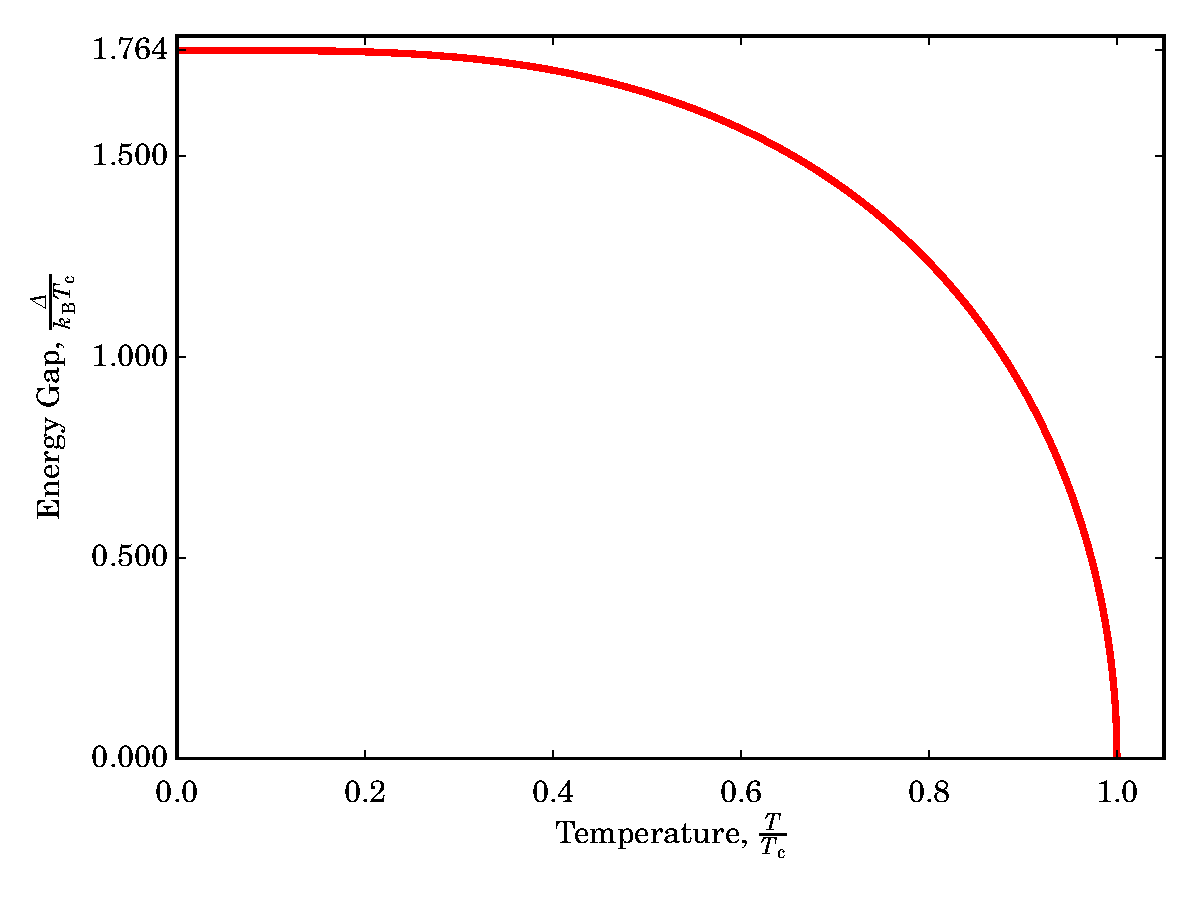
\includegraphics[width = 0.95\textwidth]{figures/BCS_gap}
\caption[BCS model of the superconducting energy gap]{Increase in the superconducting energy gap with decreasing temperature as described by \textcite{BCS1957}.}
\label{fig:BCS_gap}
\end{center}
\end{figure}
\par 
Using Equation~\ref{eqn:BCSdos} in the result from Equation~\ref{res:IVmodptfinal} gives the total number of charges, $n$, tunnelling across the barrier:
\begin{align}
n 	&= \bigintss_{-\infty}^{\infty} \frac{\left|E\right|}
														{\sqrt{\left|E\right|^{2}-\varDelta^{2}}}
		\left[\frac{1}{\e^{\frac{\left(\left|E\right| - \nicefrac{eV}{2}\right)}
		{k_{\mathrm{B}}T_{\mathrm{e}}}} + 1} - \frac{1}{\e^{\frac{\left(\left|E\right| + 
		\nicefrac{eV}{2}\right)}{k_{\mathrm{B}}T_{\mathrm{e}}}}+1} \right]\, \mathrm{d}E \,.
		\label{eqn:IVmodnfull}
%\intertext{By taking only the energies of interest, those which are positive and greater than the superconducting bandgap, Equation~\ref{eqn:IVmodnfull} can be re-written as:}
%n	&= \bigintss_{\varDelta}^{\infty} \frac{E}{\sqrt{E^{2}+\varDelta^{2}}}
%		\left[\frac{1}{\e^{\frac{\left(E - \nicefrac{eV}{2}\right)}
%		{k_{\mathrm{B}}T_{\mathrm{e}}}} + 1} - \frac{1}{\e^{\frac{\left(E + \nicefrac{eV}{2}\right)}
%		 {k_{\mathrm{B}}T_{\mathrm{e}}}}+1} \right]\, \mathrm{d}E \,. \label{eqn:IVmodnlimits}
\end{align}
Finally, it is possible to convert this number of charges into a tunnelling current, $I$, by converting Equation~\ref{eqn:IVmodnfull} to a voltage by dividing by the electron charge, $e$, and using Ohm's Law with the tunnelling resistance $R_{\mathrm{N}}$, giving:\footnote{The subscript $N$ denotes that this is the \textit{normal state} resistance of a \glsfirst{acr:IV} curve.\label{def:Rn}}
\begin{align}
I &= \frac{1}{eR_{\mathrm{N}}} n \,. 
\end{align}
Substituting the term for $n$ from Equation~\ref{eqn:IVmodnfull} gives the final result:
\begin{align}
I = 	\frac{1}{eR_{\mathrm{N}}} \bigintss_{-\infty}^{\infty}
		\frac{E}{\sqrt{E^{2}-\varDelta^{2}}}
		\left[\frac{1}{\e^{\frac{\left(E - \nicefrac{eV}{2}\right)}
		{k_{\mathrm{B}}T_{\mathrm{e}}}} + 1} - \frac{1}{\e^{\frac{\left(E + \nicefrac{eV}{2}\right)}
		{k_{\mathrm{B}}T_{\mathrm{e}}}}+1} \right]\, \mathrm{d}E \,. \label{res:IV}
\end{align}
Using this result, and if the current and the voltage of a particular device have been measured, it is possible to use a parameter fitting program to calculate the electron temperature.
\par 
Inspection of Equation~\ref{res:IV} shows that there is an exponential dependance on the electron temperature for the tunnelling current. It is this dependency which makes the tunnelling contacts described here highly sensitive thermometers. The relationship between the electron temperature and the tunnelling current (at a constant voltage bias) is shown in Figure~\ref{fig:IvsTe_model}. The tunnelling current increases rapidly with the electron temperature until the temperature of the electrons is greater than the critical temperature; at which point the tunnelling current remains constant.
\begin{figure}[t]
\begin{center}
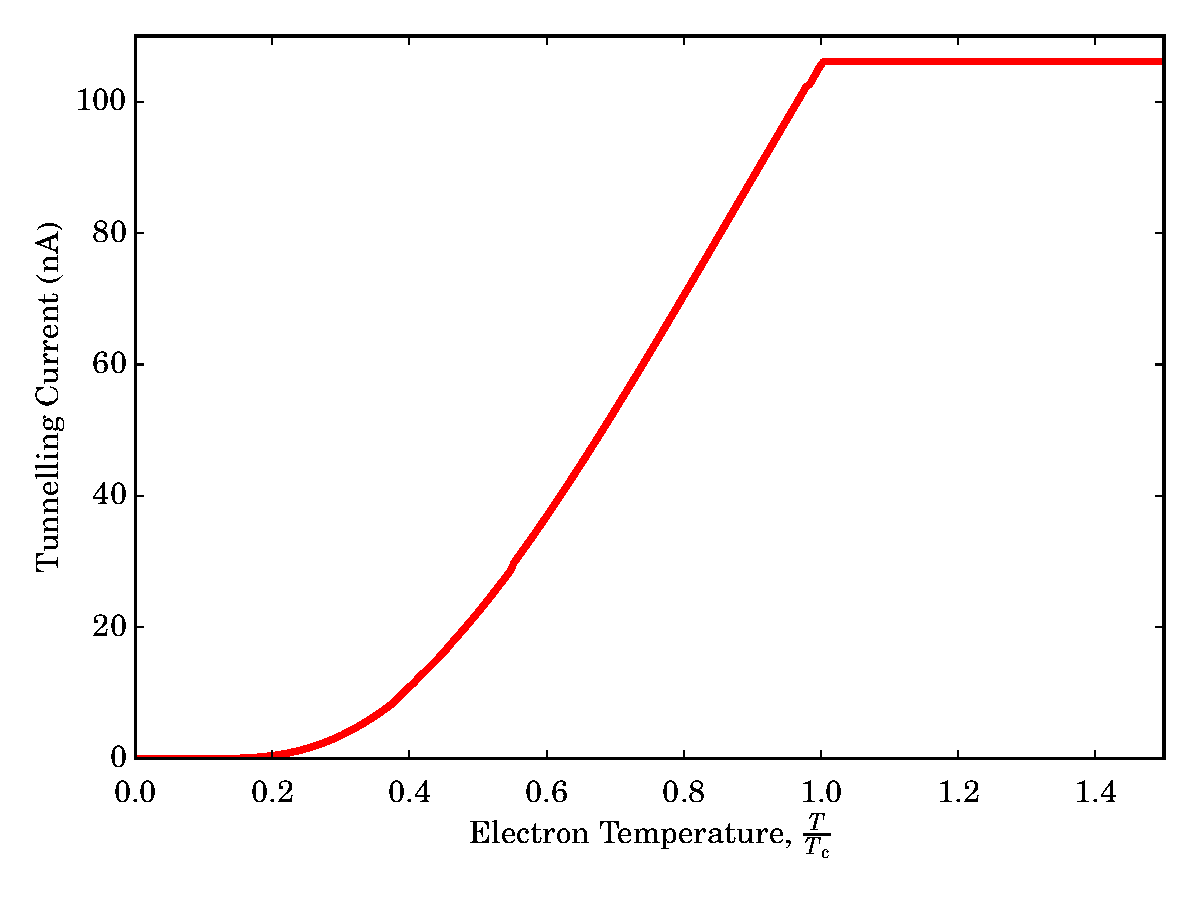
\includegraphics[width = 0.95\textwidth]{figures/IvsTe_model}
\caption[Dependance of tunnelling current on electron temperature]{The relationship between the tunnelling current and the electron temperature. This was modelled using Equation~\ref{res:IV} for a superconductor with a critical temperature of $1.2~\mathrm{K}$, biased by a voltage $V = \varDelta_{T=0}$ and a tunnelling resistance, per junction, of $1~\mathrm{k\Omega}$.}
\label{fig:IvsTe_model}
\end{center}
\end{figure}
%
\section{The Cooling Power}
\label{sec:theory-power}
Each time a charge leaves the central island by tunnelling into one of the superconducting contacts, as described in Section~\ref{sec:theory-current}, it must be replaced by a charge from one of the superconductors. When the device is biased, the most likely flow of charge will be from the semiconductor into the lower energy contact $\left(E_{\mathrm{f_{S}}} - E_{\mathrm{f_{Sm}}} = \nicefrac{-eV}{2}\right)$ and for a charge from the superconductor at a higher energy $\left(E_{\mathrm{f_{S}}} - E_{\mathrm{f_{Sm}}} = \nicefrac{eV}{2}\right)$ to fill this vacant state. This is illustrated in Figure~\ref{fig:Pmod:energyLevelsBias}. Since the charges which tunnel out are replaced by less energetic charges, the overall energy (and thus temperature) of the charges in the central island is reduced. It is this process which is utilised to create the microrefrigerator type of device \parencite{Nahum1994}. 
\begin{figure}[t]
\begin{center}
\includegraphics[height = 0.5\textheight]{figures/CEB_energyLevels_Bias}
\caption[Most likely route for charges to tunnel in a two-junction system.]{The most likely route for charges to tunnel in a biased two-junction system. If the system is biased such that the energy levels in the left hand superconductor are lowered with respect the semiconductor and the states in the right hand contact are raised (as shown), the most likely movement of charges from the semiconductor will be to above the energy gap in the left hand superconductor. This will create a vacant state, which will be filled by a charge from the top of the superconducting state in the right hand superconductor.}
\label{fig:Pmod:energyLevelsBias}
\end{center}
\end{figure}
\par
This cooling of charges in the central island of the structure can be expressed as a cooling or heating power, $P$. Depending on the exact route by which charges pass through the structure, this term will either be positive, meaning that energy is added to the semiconductor and there is net heating; or it will be negative, due to energy being removed and the temperature of the charges is lowered.
\par 
To derive an expression for this power, it is possible to follow a similar derivation to that given in Section~\ref{sec:theory-current} to find the tunnelling current (Equation~\ref{res:IV}). To do this, the probability, $p_{_{\mathrm{T}}}$, of an occupied state on one side of the barrier corresponding to a vacant state on the other is again calculated. There are four possible routes by which charges can tunnel to or from the semiconductor. These were illustrated in Figures~\ref{fig:IVmod:energyLevels-noBias}, \ref{fig:IVmod:energyLevels-+Bias} and \ref{fig:IVmod:energyLevels--Bias}. In order to calculate the total energy added to the semiconductor, each of these probabilities needs to be multiplied by the energy of the charges tunnelling. 
\begin{description}
\label{list:tunnellingEnergy}
	\item[$p_{1}$] transfers charges with energy $E+\nicefrac{eV}{2}$ from the 
			superconducting contact into the semiconductor.
	\item[$p_{2}$] transfers charges with energy 
			$-\left(E-\nicefrac{eV}{2}\right)$ from the superconductor into the 
			semiconductor.
	\item[$p_{3}$] removes charges with energy $E+\nicefrac{eV}{2}$ from the 
			central semiconductor, this means the energy contribution to the 
			semiconductor is $-\left(E+\nicefrac{eV}{2}\right)$.
	\item[$p_{4}$] removes charges with energy $-\left(E-\nicefrac{eV}{2}\right)$
			from the semiconductor, this results in an energy change of
			$E-\nicefrac{eV}{2}$ in the semiconductor.
\end{description}
\par 
To find the total energy transferred through this tunnelling $E_{\mathrm{tun}}$, the summation of these terms needs to be integrated over all energies and multiplied by the superconducting density of states, given by:
\begin{align}
N_{\mathrm{S}}\left(S\right) &= \frac{E}{\sqrt{E^{2}-\varDelta^{2}}} \,, 
\tag{\ref{eqn:BCSdos} revisited}
\end{align}This gives:
\begin{align}
E_{\mathrm{tun}} = \bigintss_{-\infty}^{\infty}
		\frac{E}{\sqrt{E^{2}-\varDelta^{2}}} 
		&\left[E\left(p_{1} - p_{2} - p_{3} + p_{4}\right)
		\vphantom{\frac{eV}{2}}\right. \nonumber \\[-0.9em] 
		&{}+\left.\frac{eV}{2}\left(p_{1} + p_{2} - p_{3} - 
		p_{4}\right)\right]\, \mathrm{d}E \,. \label{eqn:Pmod_totalE}
\end{align}
\par 
One important definition which can be taken from this is that the change in energy, due to movement of charges, is defined such that an increase in this term corresponds to the overall energy of the charges in the semiconductor increasing (i.e. heating of the charges).
\par 
To calculate the power, $P$, associated with this change in energy, Equation~\ref{eqn:Pmod_totalE} needs to be divided by the tunnelling resistance, $R_{\mathrm{N}}$, (as defined on Page~\pageref{def:Rn}) and the square of the electron charge. This additional electron charge, compared to Equation~\ref{eqn:IVmodnfull}, is the result of multiplying by the energy of the carriers as opposed to their charge. One further observation needs to be made prior to arriving at a term for the tunnelling power. When deriving Equation~\ref{res:IV} for the tunnelling current, it sufficed to examine only a single junction. This was due to the fact that since the two junctions are in a series configuration, the current through the two must be the same. In the case of the tunnelling power, heat can flow through either of the two junctions; this means that for symmetrical junctions, Equation~\ref{eqn:Pmod_totalE} needs to be further multiplied by a factor of two. This gives:
\begin{align}
P &= \frac{2}{e^{2}R_{\mathrm{N}}}
		\bigintss_{-\infty}^{\infty} \frac{E}{\sqrt{E^{2}-\varDelta^{2}}} 
		\left[E\left(p_{1} - p_{2} - p_{3} + p_{4}\right)
		\vphantom{\frac{eV}{2}}\right.  \nonumber \\[-0.9em] 
		&\qquad \qquad \qquad \qquad \qquad \quad
		{}+\left.\frac{eV}{2}\left(p_{1} + p_{2} - p_{3} - 
		p_{4}\right)\right]\, \mathrm{d}E \,. \label{eqn:Pmod_full}
\intertext{It is useful to split this in two terms, $P_{1}$ and $P_{2}$, such that:}
P_{1} &= \frac{2}{e^{2}R_{\mathrm{N}}}
		\bigintss_{-\infty}^{\infty} \frac{E}{\sqrt{E^{2}-\varDelta^{2}}} 
		\left[E\left(p_{1} - p_{2} - p_{3} + p_{4}\right)\right]
		\, \mathrm{d}E \,, \label{eqn:Pmod_P1}\\
P_{2} &= \frac{2}{e^{2}R_{\mathrm{N}}}
		\bigintss_{-\infty}^{\infty} \frac{E}{\sqrt{E^{2}-\varDelta^{2}}}
		\left[\frac{eV}{2}\left(p_{1} + p_{2} - p_{3} - p_{4}\right)\right]
		\, \mathrm{d}E \,, \label{eqn:pmod_P2} \\
P &= P_{1} + P_{2} \,. \label{eqn:Pmod_P1P2}
\intertext{Equation~\ref{eqn:pmod_P2} for $P_{2}$ can be rewritten as:}
P_{2} &= \frac{eV}{2} \frac{2}{e^{2}R_{\mathrm{N}}}
		\bigintss_{-\infty}^{\infty} \frac{E}{\sqrt{E^{2}-\varDelta^{2}}}
		\left(p_{1} + p_{2} - p_{3} - p_{4}\right)
		\, \mathrm{d}E \,, \nonumber \\
P_{2} &= V \frac{1}{eR_{\mathrm{N}}}
		\bigintss_{-\infty}^{\infty} \frac{E}{\sqrt{E^{2}-\varDelta^{2}}}
		\left(p_{1} + p_{2} - p_{3} - p_{4}\right)
		\, \mathrm{d}E \,. \label{eqn:Pmod_P2_rearr}
\intertext{By noting that tunnelling current, $I$, can be rewritten as:}
I &= 	\frac{1}{eR_{\mathrm{N}}} \bigintss_{-\infty}^{\infty}
		\frac{E}{\sqrt{E^{2}+\varDelta^{2}}}
		\left[p_{1} + p_{2} - p_{3} - p_{4}\right]\, \mathrm{d}E \,, 
		\tag{\ref{res:IV} rewritten}
\end{align}
and comparing this to Equation~\ref{eqn:Pmod_P2_rearr}, it can be seen that the latter can be simply written as:
\begin{align}
P_{2} &= IV \,. \label{res:Pmod_P2}
\end{align}
\par 
It is possible to slightly simplify Equation~\ref{eqn:Pmod_P1}, in a way similar to that performed to simplify Equation~\ref{eqn:IVmod_Pt_start} to Equation~\ref{res:IVmodptfinal} in Section~\ref{sec:theory-current}. This starts by recalling that $p_{1\mbox{--}4}$ can be written as:
\begin{align}
p_{1} &= q_{1} \times \left(1 - q_{3}\right)\,,
\tag{\ref{eqn:IVmodp1} revisited}\\
p_{2} &= q_{2} \times \left(1 - q_{4}\right)\,,
\tag{\ref{eqn:IVmodp2} revisited}\\
p_{3} &= q_{3} \times \left(1 - q_{1}\right)\,,
\tag{\ref{eqn:IVmodp3} revisited}\\
p_{4} &= q_{4} \times \left(1 - q_{2}\right)\,.
\tag{\ref{eqn:IVmodp4} revisited}
\end{align}
Thus, the term in square brackets in Equation~\ref{eqn:Pmod_P1} (which, for the sake of tidiness, we will temporarily call $A$) can be written as:
\begin{align}
A &= E\left(p_{1} - p_{2} - p_{3} + p_{4}\right)\,, \label{def:Pmod_A} \\
\therefore\, P_{1} &= \frac{2}{e^{2}R_{\mathrm{N}}}
		\bigintss_{-\infty}^{\infty} \frac{E}{\sqrt{E^{2}-\varDelta^{2}}} \times A
		\, \mathrm{d}E \,, \label{eqn:Pmod_P1_A} \\
A &= E\left(
		q_{1}\times\left(1-q_{3}\right)
		- q_{2}\times\left(1-q_{4}\right)
		{}- q_{3}\times\left(1-q_{1}\right)
		+ q_{4}\times\left(1-q_{2}\right)
		\right) \,. \label{eqn:Pmod_P1_q_start}\\
\intertext{Multiplying out these terms gives:}
A &= E\left(
		q_{1}-q_{1}q_{3}-q_{2}+q_{2}q_{4}-q_{3}+q_{3}q_{1}+q_{4}-q_{4}q_{2}
		\right) \,, \label{eqn:Pmod_P1_q_multiOut}\\
A &= E\left(q_{1}-q_{2}-q_{3}+q_{4} \right)\,.\label{eqn:Pmod_P1_q_crosscanc}\\
\intertext{This gives:}
P_{1} &= \frac{2}{e^{2}R_{\mathrm{N}}}
		\bigintss_{-\infty}^{\infty} \frac{E}{\sqrt{E^{2}-\varDelta^{2}}}
		\left[E\left(
		q_{1}-q_{2}-q_{3}+q_{4}
		\right)\right]
		\, \mathrm{d}E \,. \label{eqn:Pmod_P1_q_final}\\
\intertext{Since it is not possible to further simplify this, the final form of $P_{1}$ can be written as:}
P_{1} &= \frac{2}{e^{2}R_{\mathrm{N}}}
		\bigintss_{-\infty}^{\infty} \frac{E^{2}}{\sqrt{E^{2}-\varDelta^{2}}}
		\left[
		\frac{1}{\e^{\frac{E}{k_{\mathrm{B}}T_{\mathrm{S}}}}+1}
 		-\frac{1}{\e^{\frac{-E}{k_{\mathrm{B}}T_{\mathrm{S}}}}+1} 
		\right.  \nonumber \\
 		&\left.  \qquad \qquad \qquad \qquad \qquad \quad
		-\frac{1}{\e^{\frac{\left(E+
		\nicefrac{eV}{2}\right)}{k_{\mathrm{B}}T_{\mathrm{e}}}}+1}
		+\frac{1}{\e^{\frac{-\left(E- 
		\nicefrac{eV}{2}\right)}{k_{\mathrm{B}}T_{\mathrm{e}}}}+1} \right] \, \mathrm{d}E \,.
		\label{res:Pmod_P1}
\end{align}
\par 
Using this result, along with that of Equation~\ref{res:Pmod_P2}, in Equation~\ref{eqn:Pmod_P1P2} gives the final result of the tunnelling power as:
\begin{align}
P = IV + \frac{2}{e^{2}R_{\mathrm{N}}}
		\bigintss_{-\infty}^{\infty} \frac{E^{2}}{\sqrt{E^{2}-\varDelta^{2}}}
		&\left[
		\frac{1}{\e^{\frac{E}{k_{\mathrm{B}}T_{\mathrm{S}}}}+1}
 		-\frac{1}{\e^{\frac{-E}{k_{\mathrm{B}}T_{\mathrm{S}}}}+1} 
		\right. \nonumber \\
 		&\left.  
		{}-\frac{1}{\e^{\frac{\left(E+
		\nicefrac{eV}{2}\right)}{k_{\mathrm{B}}T_{\mathrm{e}}}}+1}
		+\frac{1}{\e^{\frac{-\left(E- 
		\nicefrac{eV}{2}\right)}{k_{\mathrm{B}}T_{\mathrm{e}}}}+1} \right] \, \mathrm{d}E \,.
		\label{res:tunnellingP}
\end{align}
%
\section{Electron-Phonon Interactions}\label{sec:eph}
As a conduction electron moves through a material, such as the lattice of a semiconductor, it will experience interaction with the ion cores created by the vacation of electrons. The simplest result of these interactions is the scattering of electrons due to collisions with the lattice as they move through the lattice, this is the origin of electrical resistance. These collisions result in an exchange of energy between the electrons and phonons, which can be expressed as a thermal conduction, $G_{\mathrm{e\mbox{-}ph}}$, between the two systems. As will be seen later in this section, this thermal conduction plays a large part in determining the limit of a cold-electron bolometer's sensitivity.
\par 
The fluctuation-dissipation theorem presented by \textcite{Nyquist1928b} shows that this thermal conduction will have fluctuations on the order of $k_{\mathrm{B}}T$ and having a power spectral density of $S_{G} = 4k_{\mathrm{B}}T^{2}G$. From this, it is clear that the energy transferred between an electron and a phonon in a collision is directly proportional to temperature in the case of a \textit{clean} metal or $T^{2}$ in a \textit{dirty} thin-film metal or highly-doped semiconductor , where there are a large number of impurities. Further dependencies of the power on temperature arise from the rate of collision between the electrons and the phonons \parencite[see][]{Ziman2001}, which contributes an additional dependency on $T$, and the Bose-Einstein distribution governing the number of states filled, which yields a further $T^{3}$ dependency. In total, it has been shown that for a metal, the power flow between the two systems depends on the temperature to the power $5$ \parencite{Ziman2001}, whereas for a degenerately-doped semiconductor, the dependance has a $T^{6}$ relationship \parencite{Prunnila2007}, as will be used later in this chapter.
\par 
These relatively high-order dependencies on the temperature indicate clearly that at low temperatures, one should expect the interaction between the two systems to be weak. When the electrons and phonons are at different temperatures, these collisions will result in a net flow of power from the more energetic (hotter) system to the other. This power flow is given by:
\begin{align}
P = \varSigma\varOmega\left(T_{\mathrm{e}}^{\beta} - T_{\mathrm{ph}}^{\beta}\right)\,,
\label{eqn:e-phPower}
\end{align}
where $\varOmega$ is the volume of the material in which the collisions occur, $T_{\mathrm{e}}$ and $T_{\mathrm{ph}}$ are the temperature of the electrons and phonons respectively, $\beta$ is the power dependency of the interactions on temperature (nominally $5$ for a metal and $6$ for a highly-doped semiconductor, as already discussed), and $\varSigma$ is a material parameter. \textcite{Wellstood1994} present a approximation for $\varSigma$ for a metal ($\beta = 5$) given by:
\begin{align}
\varSigma = \frac{\hbar}{2\rho c_{\mathrm{s}}}
	\left(\frac{2E_{\mathrm{F}}}{3}\right)^{2}
	\frac{D\left(E_{\mathrm{F}}\right)k_{\mathrm{B}}^{5}
		\Gamma\left(5\right)\upzeta\left(5\right)}
		{2\pi\hbar^{5}c_{\mathrm{s}}^{3}v_{\mathrm{F}}\Omega}\,,
\label{eqn:sigma}
\end{align}
where $\rho$ lattice density, $c_{\mathrm{s}}$ is the speed of sound in the lattice, $E_{\mathrm{F}}$ and $v_{\mathrm{F}}$ are the Fermi energy and velocity, $D\left(E\right)$ is the density of states at energy $E$, and $\Gamma$ and $\upzeta$ are the Gamma and Riemann zeta functions respectively. It should, however, be noted that when tested by \textcite{Wellstood1994} and \textcite{Qu2005}, both found that the model presented in Equation~\ref{eqn:sigma} produced values differing by in excess of an order of magnitude compared  to measured values and thus it is concluded that Equation~\ref{eqn:sigma} produces, at best, a rough approximation of $\varSigma$.
\par 
\textcite{Muhonen2011} present a discussion of the effect of straining a semiconductor's lattice on the interaction between electrons and phonons. A simplistic interpretation of their results is that, as strain is introduced in two dimensions of the lattice (the in-plane dimensions), the energy levels for interactions between the in-plane atoms and electrons are increased with strain, to the degree that they are effectively depopulated and electrons only interact via the out-of-plane energy bands (which are not affected by the straining of the lattice). \citeauthor{Muhonen2011} tested two materials, one with a straining layer consisting of \ce{Si_{0.8}Ge_{0.2}} (resulting in a strain factor of around $0.95~\%$ in the doped silicon), and one unstrained control sample. Both samples used silicon doped with phosphorus to a concentration of $4 \times 10^{19}~\mathrm{cm^{-3}}$. Note that these two materials are, to all intents and purposes, identical to the materials used to fabricate the devices examined in this work. Examining the same samples, \textcite{Prest2011} found that the strained material showed substantially weaker coupling of the electrons and phonons compared to the unstrained control sample, with a $\Sigma$ value of $2 \times 10^{7}~\mathrm{W\,K^{-6}\,m^{-3}}$ for the strained material and $5.2 \times 10^{8}~\mathrm{W\,K^{-6}\,m^{-3}}$ for the control sample. This is also shown by \textcite{Muhonen2011} who, while not calculating values of $\Sigma$, do present graphs of $G_{\mathrm{e\mbox{-}ph}}$ vs $T_{\mathrm{e}}$ for both materials in Figure~2b of their manuscript. \citeauthor{Muhonen2011} explain that the power loss in interactions between the electrons and phonons can be expressed as:
\begin{align}
P_{\mathrm{e\mbox{-}ph}} = F\left(T_{\mathrm{e}}\right) 
	- F\left(T_{\mathrm{ph}}\right)\,, \label{eqn:ephPowerLoss}
\end{align}
where $F\left(T\right)$ is the energy loss function, which, according to \textcite{Prunnila2007}, may be written as:
\begin{align}
F\left(T\right) = F_{\mathrm{S}}\left(T\right) + F_{\mathrm{A}}\left(T\right)\,,
\end{align}
where $F_{\mathrm{S}}\left(T\right)$ and $F_{\mathrm{A}}\left(T\right)$ are the symmetric and asymmetric parts of the energy loss function. Following the rigorous mathematical treatment presented by \textcite{Prunnila2007}, \citeauthor{Muhonen2011} show that, for their control sample, both the symmetric and asymmetric components contribute to the energy loss function and, furthermore, it can be said that $F_{\mathrm{A}} \gg F_{\mathrm{S}}$ and thus for the unstrained sample:
\begin{align}
G_{\mathrm{e\mbox{-}ph}} \approx
	\frac{\partial F_{\mathrm{A}}}{\partial T_{\mathrm{e}}}\,.
\label{eqn:controlG}
\end{align}
They go on to explain that, if the in-plane energy bands are fully depopulated, then $F_{\mathrm{A}} = 0$ and thus the thermal conduction between the electrons and phonons in the strained device (under this assumption) is given by:
\begin{align}
G_{\mathrm{e\mbox{-}ph}} = 
	\frac{\partial F_{\mathrm{S}}}{\partial T_{\mathrm{e}}}\,,
\label{eqn:strainG}
\end{align}
which, when computed, is found to be a factor of several thousand times smaller than the result of Equation~\ref{eqn:controlG}. Looking at the results presented in Figure~2b of \textcite{Muhonen2011}, it is clear that Equation~\ref{eqn:controlG} produces a close fit to their experimental results. However, the results for the strained sample agree with Equation~\ref{eqn:strainG} only in that $G_{\mathrm{e\mbox{-}ph}}$ is less for the strained material compared to the control. The magnitude of the reduction is only a factor 20--50 across the entire temperature range studied ($0.2\mbox{--}0.5~\mathrm{K}$). This is many orders of magnitude less than the change predicted by Equation~\ref{eqn:strainG}. From this, it can be concluded that the in-plane energy bands have not been fully depopulated at this level of strain and the assumption that $F_{\mathrm{A}} = 0$ does not hold. This also implies that there is a great deal of potential to decrease the electron-phonon coupling further through the introduction of additional strain into the doped silicon. At the time of writing, this has not been explored and the materials used in this work are essentially identical to those described by \textcite{Muhonen2011} and \textcite{Prest2011}.
%
\section{The Responsivity}
\label{sec:theory-responsivity}
Like all bolometric detectors, it is possible to bias a cold-electron bolometer with either a voltage or a current. In either case, the quantity which is not providing the bias is monitored and it is in this signal that the response to a change in incident optical power will be measured. The responsivity, $S$, of a detector is defined as the ratio of the change in the measured signal to the change in the power absorbed in the detector. This is written as:
\begin{align}
S &= \frac{\d\mathit{signal}}{\mathrm{d}P_{\mathrm{abs}}} \,, \label{def:responsivity}
\intertext{where $\mathit{signal}$ is the quantity being monitored and $P_{\mathrm{abs}}$ is the absorbed power. Since a bolometric detector is biased by either a voltage or a current, we can define two types of responsivity. In the case of a voltage-biased detector, where the current flowing through the detector is monitored, the current responsivity, $S_{\mathrm{I}}$, is given by:}
S_{\mathrm{I}} &= \frac{\mathrm{d}I}{\mathrm{d}P_{\mathrm{abs}}} \,, \label{def:responsivityI}
\intertext{where $I$ is the current being measured. For a detector biased by a current, the voltage responsivity, $S_{\mathrm{V}}$, is given by:}
S_{\mathrm{V}} &= \frac{\mathrm{d}V}{\mathrm{d}P_{\mathrm{abs}}} \,, \label{def:responsivityV}
\end{align}
where $V$ is the measured voltage.
\par 
These terms are general expressions and need to be rewritten such that their values can be calculated. In order to derive useful expressions for the responsivity, it is important to understand the relative contributions to the heating (or cooling) of the electrons in the detector's absorber. Along with tunnelling power (Equation~\ref{res:tunnellingP}), which adds or removes heat via the tunnelling current, the electrons in the absorber are also affected by various other sources of heating or cooling. The most significant of which are: Joule heating, $P_{\mathrm{J}}$, due the resistance experienced by the current within the absorber; the energy from a radiative source which is absorbed by the detector, $P_{\mathrm{abs}}$; and the flow of energy directly between the electron and the phonon systems, $P_{\mathrm{e\mbox{-}ph}}$. Joule heating was first described by \textcite{Joule1837}; it is caused by the collisions between the charges flowing in the current and the atomic ions in the conductor. The heating power from these collisions is given by:
\begin{align}
P_{\mathrm{J}} &= I^{2}R\,, \label{def:JouleHeating}
\end{align}
where $I$ is the current flowing through a resistance $R$.
\par 
Unless the electron and phonon systems are at thermal equilibrium, there will be a flow of heat between the two due to the thermal link between the systems. The heating (or cooling) power resulting from this flow of heat is given by:
\begin{align}
P_{\mathrm{e\mbox{-}ph}} &= \varSigma \varOmega\left(T_{\mathrm{e}}^{\beta} 
	- T_{\mathrm{ph}}^{\beta}\right)\,, \label{def:e-phPower}
\end{align}
where $\varSigma$ is a material constant relating to how strong the thermal link between the electrons and phonons is; $\varOmega$ is the volume in which the electrons and phonons are not in thermal equilibrium; $T_{\mathrm{e}}$ and $T_{\mathrm{ph}}$ are the temperatures of the electrons and the phonons respectively; and $\beta$ is the power dependance on the temperature of the heat flow. Unlike all of the other terms mentioned (including the tunnelling power), this term is positive for the removal of energy (cooling) from the electrons and negative for heating of the electrons.
\par 
For the absorber to be at a constant temperature, these terms must add up to zero. This is referred to as the heat balance equation (or the heat balance condition) and can be expressed as:
\begin{align}
P + P_{\mathrm{abs}} + P_{\mathrm{J}} - P_{\mathrm{e\mbox{-}ph}} = 0 \,, \label{eqn:heatBalance}
\end{align}
where $P$ is the tunnelling power given in Equation~\ref{res:tunnellingP} (note that $P$ is negative for electron cooling); $P_{\mathrm{abs}}$ is the power absorbed in the detector due to incident optical power; $I$ is the current flowing through the absorber of the detector; $R_{\mathrm{abs}}$ is the resistance of the detector's absorber; $\varSigma$ is the material constant of the absorber; $\varOmega$ is the volume of the absorber; $T_{\mathrm{e}}$ and $T_{\mathrm{ph}}$ are the temperatures of the electrons and phonons respectively; and $\beta$ is the power of temperature dependency of electron-phonon cooling power, this has been found by \textcite{Prest2011} to be $6$. This equation is simply the equilibrium condition for the temperature of the electrons in the absorber; the first three terms are defined as being positive for heating of the electrons, whereas the final term is defined as being positive for cooling of the charges. The meaning of the first two terms has already been covered, the third term is simply the Joule heating of the electrons in the absorber due to the current flowing through the absorber. The final term is the cooling of the electrons due to their thermal link to the phonons; this is positive when the temperature of the phonons is less than that of the electrons and is thus a cooling power as opposed to a heating power.
\par 
In the case of a voltage-biased detector, the current responsivity, $S_{\mathrm{I}}$, can be derived by noting that Equation~\ref{def:responsivityI} can be rewritten as:
\begin{align}
S_{\mathrm{I}} &= \frac{\mathrm{d}I}{\mathrm{d}P_{\mathrm{abs}}} 
		 = \frac{\frac{\mathrm{\partial}I}{\mathrm{\partial}T_{\mathrm{e}}}}
				{\frac{\mathrm{\partial}P_{\mathrm{abs}}}{\mathrm{\partial}T_{\mathrm{e}}}}\,. 
	\label{eqn:SmodIresponStart}
\intertext{The denominator of this can be found by differentiating the heat balance equation (Equation~\ref{eqn:heatBalance}).}
0 &= \frac{\partial P}{\partial T_{\mathrm{e}}} 
		+ \frac{\partial P_{\mathrm{abs}}}{\partial T_{\mathrm{e}}}
		+ \frac{\partial}{\partial T_{\mathrm{e}}}I^{2}R_{\mathrm{abs}}
		-  \beta \varSigma \varOmega T_{\mathrm{e}}^{\beta-1}\,, \\
\frac{\partial P_{\mathrm{abs}}}{\partial T_{\mathrm{e}}} 
	&= \beta \varSigma \varOmega T_{\mathrm{e}}^{\beta-1} 
		- \frac{\partial P}{\partial T_{\mathrm{e}}}
		- \frac{\partial}{\partial T_{\mathrm{e}}}I^{2}R_{\mathrm{abs}} \,. 
	\label{eqn:SmoddHBdT_Vbias}
\intertext{Substituting this result into Equation~\ref{eqn:SmodIresponStart} gives the final result:}
S_{\mathrm{I}} &= \frac{\frac{\mathrm{\partial}I}{\mathrm{\partial}T_{\mathrm{e}}}}
		{\beta \varSigma \varOmega T_{\mathrm{e}}^{\beta-1} 
		- \frac{\partial P}{\partial T_{\mathrm{e}}}
		- \frac{\partial}{\partial T_{\mathrm{e}}}I^{2}R_{\mathrm{abs}}} \,. 
	\label{res:Iresponsivity}
\end{align}
This differs slightly from Equation 10 of \textcite{Golubev2001}, who do not consider the Joule heating of the absorber in their model but who do consider the effects of operating in an AC regime.\footnote{Also note that \citeauthor{Golubev2001} define the tunnelling power to be positive for cooling of the electrons.}
\par 
It is possible to derive the voltage responsivity ($S_{\mathrm{V}}$) similarly, by starting with:
\begin{align}
S_{\mathrm{V}} &= \frac{\mathrm{d}V}{\mathrm{d}P_{\mathrm{abs}}} 
		 = \frac{\frac{\partial V}{\partial T_{\mathrm{e}}}}
				{\frac{\mathrm{\partial}P_{\mathrm{abs}}}{\mathrm{\partial}T_{\mathrm{e}}}}\,. 
	\label{eqn:SmodVresponStart}
\end{align}
Since, in the current-biased regime, the current across the detector cannot change it is possible to write:
\begin{align}
\frac{\mathrm{d}I}{\mathrm{d}T_{\mathrm{e}}} &= 0
		= \frac{\partial I}{\partial V}\frac{\partial V}{\partial T_{\mathrm{e}}} 
			+ \frac{\partial I}{\partial T_{\mathrm{e}}} \,, \\
\frac{\partial V}{\partial T_{\mathrm{e}}} 
		&= \frac{-\frac{\partial I}{\partial T_{\mathrm{e}}}}
				{\frac{\partial I}{\partial V}} \,. \label{eqn:SmoddVdTrearr} 
\end{align}
Using this in the numerator of Equation~\ref{eqn:SmodVresponStart} yields:
\begin{align}
S_{\mathrm{V}} &=  \frac{\frac{-\frac{\partial I}{\partial T_{\mathrm{e}}}}
				{\frac{\partial I}{\partial V}}}
				{\frac{\mathrm{\partial}P_{\mathrm{abs}}}{\mathrm{\partial}T_{\mathrm{e}}}}\,. 
	\label{eqn:SmodVresponNumSub}
\end{align}
As in the case for the current responsivity, the numerator can be found by differentiating the heat balance equation. In the current-biased regime, there are two subtle differences to that of Equation~\ref{eqn:SmoddHBdT_Vbias}. The first being that the Joule heating term no longer depends on the electron temperature, since the current is constant and thus:
\begin{align}
\left(\frac{\partial}{\partial T_{\mathrm{e}}} I^{2}R_{\mathrm{abs}}\right)_{I} &= 0 \,.
			\label{eqn:SmodJouleHeatingIbias}
\end{align}
The second is the that the tunnelling power (given by Equation~\ref{res:tunnellingP}) is a function of both the electron temperature and the voltage (along with the temperature of the charges in the superconductor). In the voltage-biased case, the voltage was not a function of the electron temperature. In the current-bias regime, since the current is fixed, the voltage across the tunnelling contacts must vary with the temperature of the charges, this means that:
\begin{align}
\frac{\mathrm{d}P}{\mathrm{d}T_{\mathrm{e}}}
		&= \frac{\partial P}{\partial V}\frac{\partial V}{\partial T_{\mathrm{e}}}
			+ \frac{\partial P}{\partial T_{\mathrm{e}}} \,.
\intertext{Substituting the result of Equation~\ref{eqn:SmoddVdTrearr} gives:}
\frac{\mathrm{d}P}{\mathrm{d}T_{\mathrm{e}}}
		&= \frac{\partial P}{\partial T_{\mathrm{e}}}
			- \frac{\frac{\partial I}{\partial T_{\mathrm{e}}}}
				{\frac{\partial I}{\partial V}}\frac{\partial P}{\partial V} \,.
\end{align}
Noting this, along with the differential of the Joule heating power from Equation~\ref{eqn:SmodJouleHeatingIbias}, the differential of the heat balance equation is now:
\begin{align}
0 &= \frac{\partial P_{\mathrm{abs}}}{\partial T_{\mathrm{e}}}
		+\frac{\partial P}{\partial T_{\mathrm{e}}}
		- \frac{\frac{\partial I}{\partial T_{\mathrm{e}}}}
				{\frac{\partial I}{\partial V}}\frac{\partial P}{\partial V}
		-  \beta \varSigma \varOmega T_{\mathrm{e}}^{\beta-1}\,,
\intertext{giving:}
\frac{\partial P_{\mathrm{abs}}}{\partial T_{\mathrm{e}}} 
	&= \beta \varSigma \varOmega T_{\mathrm{e}}^{\beta-1}
		+ \frac{\frac{\partial I}{\partial T_{\mathrm{e}}}}
				{\frac{\partial I}{\partial V}}\frac{\partial P}{\partial V}
		- \frac{\partial P}{\partial T_{\mathrm{e}}} \,. 
	\label{eqn:SmoddHBdT_Ibias}
\end{align}
Substituting this for the denominator of Equation~\ref{eqn:SmodVresponNumSub} gives the final form of the voltage responsivity to be:
\begin{align}
S_{\mathrm{V}} &=  \frac{\frac{-\frac{\partial I}{\partial T_{\mathrm{e}}}}
				{\frac{\partial I}{\partial V}}}
				{\beta \varSigma \varOmega T_{\mathrm{e}}^{\beta-1} 
				+ \frac{\frac{\partial I}{\partial T_{\mathrm{e}}}}
					{\frac{\partial I}{\partial V}}\frac{\partial P}{\partial V}
				- \frac{\partial P}{\partial T_{\mathrm{e}}}}\,. \label{res:Vresponsivity} 
\end{align}
This is the same, in the DC limit, as Equation~30 of \textcite{Golubev2001}.

\section{The Sources of Electrical Noise}
\label{sec:theory-noise}
In order for incoming optical radiation to be measured by a detector system, the output signal produced must be greater than the noise signal of the detector or the readout system used. This means that a detector with a high level of inherent noise is less sensitive than a detector with a lower level of noise. When developing a detector, there are two main goals. The first is to prove that the underlying principles are in fact valid and that a functioning detector can be made. The second is to make the detector as sensitive as possible.\footnote{It is worth mentioning that, depending upon the desired application for a detector, improvements to the detector's speed may be as desirable as improved sensitivity, if not even more so.} Because of this, it is important to have a strong understanding of the noise processes involved in a detector.
\par 
There are several physical phenomena that cause noise. These can be roughly grouped into two categories: noise due to some form of fluctuation and noise resulting from the contamination of one signal by another. It is usually possible to shield electrical wiring and components to eliminate contamination of a signal, however, some sources may be more problematic to remove; for example $50~\mathrm{Hz}$ or \textit{mains noise} is caused by the switching AC voltage used to power electrical equipment and, since it is most likely essential to use some form of mains-powered equipment to monitor a detector, this noise may prove impossible to fully eradicate. Noise due to fluctuations in the energy of the charges within the detector are inevitable and can, at best, only be partially reduced through cleverly designing the detector or the materials used.
\par  
In deriving a term for the expected noise measured for a silicon cold-electron bolometer, three types of noise will be considered. Firstly, internal noise within the detector; these terms are due to various internal factors which cause the energy of the charges to fluctuate. Secondly, noise which is the result of incident power absorbed by the device. Finally, amplifier or readout noise, which is added to the signal by the electronic systems used to monitor the detector. It is worth noting here that (as will be seen in Chapter~\ref{cha:readout}) the noise of an amplifier, or the readout system as a whole, is often higher at low frequencies (typically below $10~\mathrm{Hz}$) due to so called $\nicefrac{1}{f}$ noise, whose origin is not well understood.
\par 
For the internal noise, two contributions will be considered; these are the current shot noise $\left<\delta I\right>$ and the power or heat-flow noise $\left<\delta P\right>$. As can be seen from Section~\ref{sec:theory-power} (and particularly Equation~\ref{res:tunnellingP}), these two quantities are not uncorrelated; indeed, the tunnelling power depends heavily on the current (as one might expect). To address this correlation between these two quantities, a third term, the correlated noise, $\left<\delta P \delta I\right>$, is introduced.
\par 
For these terms, the fluctuations that cause the corresponding noise will be taken to be governed by Poisson statistics, meaning that:
\begin{align}
\sigma_{x} = \sqrt{\bar{x}}\,, \label{def:PoissonStats}
\end{align}
where $\sigma_{x}$ is the standard deviation of the quantity $x$ and $\bar{x}$ is the mean value of $x$.
\par 
In the case of the current shot noise, the generated noise is due to the fluctuations in the number of electrons tunnelling across the Schottky contacts. The total number of charges, $n$, tunnelling (in any direction) for a two-junction system is given by:
\begin{align}
n &=2  \bigintss_{-\infty}^{\infty}\frac{E} 
		{\sqrt{E^{2}-\varDelta^{2}}}\left[p_{1} + p_{2} + p_{3} + 
		p_{4}\right]\,\mathrm{d}E \,,
\intertext{where $p_{1\mbox{--}4}$ are the terms defined on Page~\pageref{eqn:IVmodp1}; the factor of two comes from the fact that charges can tunnel through two junctions. This can be converted to a total noise current, $I_{\mathrm{N}}$, by dividing by the electron charge and the tunnelling resistance to give:}
I_{\mathrm{N}} &=\frac{2}{e R_{\mathrm{N}}}\bigintss_{-\infty}^{\infty}\frac{E} 
		{\sqrt{E^{2}-\varDelta^{2}}}\left[p_{1} + p_{2} + p_{3} + 
		p_{4}\right]\,\mathrm{d}E \,. \label{eqn:NmodNoiseCurrent}
\end{align}
\textcite{Schottky1918} provides the general formula for the current shot noise due to the flow of current to be:
\begin{align}
\left<\delta I\right> &= \sqrt{2eI} \,. \label{eqn:SchottkyNoise}
\end{align}
Substituting the noise current from Equation~\ref{eqn:NmodNoiseCurrent} gives the final equation for the current shot noise, due to current flow, to be:
\begin{align}
\left<\delta I^{2}\right> &= \frac{4}{R_{\mathrm{N}}}\bigintss_{-\infty}^{\infty}\frac{E} 
		{\sqrt{E^{2}-\varDelta^{2}}}\left[p_{1} + p_{2} + p_{3} + p_{4}\right]
		\,\mathrm{d}E \,,
\intertext{or more completely:}
\left<\delta I^{2}\right> &= \frac{4}{R_{\mathrm{N}}}\bigintss_{-\infty}^{\infty}\frac{E} 
		{\sqrt{E^{2}-\varDelta^{2}}}\left[
		\frac{1}{\e^{\frac{E}{k_{\mathrm{B}}T_{\mathrm{S}}}}+1} +
		\frac{1}{\e^{\frac{-E}{k_{\mathrm{B}}T_{\mathrm{S}}}}+1} +
		\frac{1}{\e^{\frac{\left(E+
						\nicefrac{eV}{2}\right)}{k_{\mathrm{B}}T_{\mathrm{e}}}}+1} \nonumber \right. \\
		&\left. \qquad \qquad \qquad +\frac{1}{\e^{\frac{-\left(E- 
						\nicefrac{eV}{2}\right)}{k_{\mathrm{B}}T_{\mathrm{e}}}}+1} -
		2\frac{1}{\e^{\frac{E}{k_{\mathrm{B}}T_{\mathrm{S}}}}+1}
				\frac{1}{\e^{\frac{\left(E+
						\nicefrac{eV}{2}\right)}{k_{\mathrm{B}}T_{\mathrm{e}}}}+1} \nonumber \right. \\
		&\left. \qquad \qquad \qquad \qquad \qquad \qquad  -2 
				\frac{1}{\e^{\frac{-E}{k_{\mathrm{B}}T_{\mathrm{S}}}}+1}
				\frac{1}{\e^{\frac{-\left(|E- 
						\nicefrac{eV}{2}\right)}{k_{\mathrm{B}}T_{\mathrm{e}}}}+1}
		\right] \,\mathrm{d}E \,. \label{res:CurrentNoise}
\end{align}
\par 
The noise due to the flow of heat, either into or from the semiconducting absorber, is derived similarly. As was the case when deriving Equation~\ref{res:tunnellingP} for the tunnelling power, the power (or heat-flow) noise is essentially the current shot noise multiplied by the energy of the charges tunnelling.
\par
As previously covered on Page~\pageref{list:tunnellingEnergy} of Section~\ref{sec:theory-power}, each of the tunnelling routes (shown on Page~\pageref{fig:IVmod:energyLevels-noBias}) contributes a different amount of energy (per charge tunnelling) to the semiconductor. To recap, the energy change in the semiconductor due to each of the four routes is:
\begin{description} \label{list:Nmod_tunnellingEnergySum}
	\item{Route 1} causes an energy change of $E+\nicefrac{eV}{2}$,
	\item{Route 2} causes an energy change of $-\left(E-\nicefrac{eV}{2}\right)$,
	\item{Route 3} causes an energy change of $-\left(E+\nicefrac{eV}{2}\right)$,
	\item{Route 4} causes an energy change of $E-\nicefrac{eV}{2}$.
\end{description}
\par
As was the case when calculating the current shot noise, it is only the magnitude of the fluctuations in the tunnelling power that are of interest when calculating the noise. This means that to find to power (heat-flow) noise, $P_{\mathrm{N}}$, Equation~\ref{eqn:Pmod_full} can be rewritten as:
\begin{align}
P_{\mathrm{N}} &= \frac{2}{e^{2}R_{\mathrm{N}}}
		\bigintss_{-\infty}^{\infty} \frac{E}{\sqrt{E^{2}-\varDelta^{2}}} 
		\left[E\left(p_{1} + p_{2} + p_{3} + p_{4}\right)
		\vphantom{\frac{eV}{2}}\right.  \nonumber \\[-0.9em] 
		&\qquad \qquad \qquad \qquad \qquad \quad
		{}+\left.\frac{eV}{2}\left(p_{1} - p_{2} + p_{3} - 
		p_{4}\right)\right]\, \mathrm{d}E \,. \label{eqn:Nmod_Pnoise_start}
\end{align}
As explained by \textcite{Golubev2001}, the heat-flow noise, $\left<\delta P\right>$, is given by:
\begin{align}
\left<\delta P\right> &= \sqrt{2EP_{\mathrm{N}}}\,. \label{eqn:Nmod_GolubevPnoise}
\end{align}
This is the same as Equation~\ref{eqn:SchottkyNoise} for the current shot noise but the electron charge ($e$) is replaced by the energy ($E$) which is fluctuating. Combining these two equations gives the heat-flow noise:
\begin{align}
\left<\delta P^{2}\right> &= \frac{4}{e^{2}R_{\mathrm{N}}}
		\bigintss_{-\infty}^{\infty} \frac{E}{\sqrt{E^{2}-\varDelta^{2}}} 
		\left[E^{2}\left(p_{1} + p_{2} + p_{3} + p_{4}\right)
		\vphantom{\frac{eV}{2}}\right.  \nonumber \\[-0.9em] 
		&\qquad \qquad \qquad \qquad \qquad \quad
		{}+\left.\left(\frac{eV}{2}\right)^{2}\left(p_{1} - p_{2} + p_{3} - 
		p_{4}\right)\right]\, \mathrm{d}E \,.
\intertext{Substituting for $p_{1\mbox{--}4}$ gives the complete result:}
\left<\delta P^{2}\right> &= \frac{4}{e^{2}R_{\mathrm{N}}}
		\bigintss_{-\infty}^{\infty} \frac{E}{\sqrt{E^{2}-\varDelta^{2}}}
		\left[E^{2}\left(
		\frac{1}{\e^{\frac{E}{k_{\mathrm{B}}T_{\mathrm{S}}}}+1} +
		\frac{1}{\e^{\frac{-E}{k_{\mathrm{B}}T_{\mathrm{S}}}}+1} +
		\frac{1}{\e^{\frac{\left(E+
						\nicefrac{eV}{2}\right)}{k_{\mathrm{B}}T_{\mathrm{e}}}}+1} \nonumber	
																				\right. \right. \\
		&\left.\left. \qquad \qquad \qquad +\frac{1}{\e^{\frac{-\left(E- 
						\nicefrac{eV}{2}\right)}{k_{\mathrm{B}}T_{\mathrm{e}}}}+1} +
		2\frac{1}{\e^{\frac{E}{k_{\mathrm{B}}T_{\mathrm{S}}}}+1}
				\frac{1}{\e^{\frac{\left(E+
						\nicefrac{eV}{2}\right)}{k_{\mathrm{B}}T_{\mathrm{e}}}}+1} \nonumber	
																				\right. \right. \\
		&\left.\left. \qquad \qquad \qquad \qquad \qquad \qquad  +2 
				\frac{1}{\e^{\frac{-E}{k_{\mathrm{B}}T_{\mathrm{S}}}}+1}
				\frac{1}{\e^{\frac{-\left(|E- 
						\nicefrac{eV}{2}\right)}{k_{\mathrm{B}}T_{\mathrm{e}}}}+1} \right) \nonumber 
																							\right. \\ 
		&\left. \qquad \qquad \qquad + \left(\frac{eV}{2}\right)^{2} \left(
		\frac{1}{\e^{\frac{E}{k_{\mathrm{B}}T_{\mathrm{S}}}}+1} -
		\frac{1}{\e^{\frac{-E}{k_{\mathrm{B}}T_{\mathrm{S}}}}+1} +
		\frac{1}{\e^{\frac{\left(E+
						\nicefrac{eV}{2}\right)}{k_{\mathrm{B}}T_{\mathrm{e}}}}+1} \nonumber	
																				\right. \right. \\
		&\left.\left. \qquad \qquad \qquad -\frac{1}{\e^{\frac{-\left(E- 
						\nicefrac{eV}{2}\right)}{k_{\mathrm{B}}T_{\mathrm{e}}}}+1} +
		2\frac{1}{\e^{\frac{E}{k_{\mathrm{B}}T_{\mathrm{S}}}}+1}
				\frac{1}{\e^{\frac{\left(E+
						\nicefrac{eV}{2}\right)}{k_{\mathrm{B}}T_{\mathrm{e}}}}+1} \nonumber	
																				\right. \right. \\
		&\left.\left. \qquad \qquad \qquad \qquad \qquad \qquad  -2 
				\frac{1}{\e^{\frac{-E}{k_{\mathrm{B}}T_{\mathrm{S}}}}+1}
				\frac{1}{\e^{\frac{-\left(|E- 
						\nicefrac{eV}{2}\right)}{k_{\mathrm{B}}T_{\mathrm{e}}}}+1} 
		\right) \right] \, \mathrm{d}E \,. \label{res:powerNoise}
\end{align}
\par 
When combining the noise sources, it is important to note that the current shot noise and the heat-flow noise are correlated, since the tunnelling power depends heavily on the current flowing through the junctions. As such, the total noise resulting from these two sources is not simply given by adding them in quadrature; instead a third term, the cross-correlator, needs to be added. For two correlated noise sources ($e_{1}$ and $e_{2}$), the total noise, $e_{\mathrm{T}}$ can be found by:
\begin{align}
e_{\mathrm{T}}^{2} &= e_{1}^{2} + e_{2}^{2} + 2Ce_{1}e_{2}\,, \label{eqn:addingCorrNoise}
\end{align}
where the dimensionless constant $C$ is the \textit{correlation coefficient} which varies between $-1$ (if the two sources are anti-correlated) and $+1$ (if the two sources are perfectly correlated). This means the correlator (the final term in Equation~\ref{eqn:addingCorrNoise}) of the current and heat-flow noise sources, $\left<\delta P \delta I\right>$, is given by:
\begin{align}
\left<\delta P \delta I\right> &= 2C\left<\delta P\right>\left<\delta I\right>
	\,.
\end{align}
The current shot noise and the heat-flow noise have been shown by \textcite{Golwala1997} to be anti-correlated so $C=-1$. Using this result and Equations~\ref{eqn:SchottkyNoise} and \ref{eqn:Nmod_GolubevPnoise} gives the correlator of the current shot and heat-flow noise to be:
\begin{align}
\left<\delta P \delta I\right> &= -4\sqrt{eEI_{\mathrm{N}}P_{\mathrm{N}}}\,. \label{eqn:NmodPInoise}
\end{align}
\textcite{Golubev2001} show that, in the case $T_{\mathrm{e}} = T_{\mathrm{S}}$, the above can be simplified to:
\begin{align}
\left<\delta P \delta I\right> &= -4eP \,. \label{eqn:NmodPInoise_Golubev}
\end{align}
Substituting Equation~\ref{res:tunnellingP} for tunnelling power gives the result:
\begin{align}
\left<\delta P \delta I\right> = -4eIV - \frac{8}{e R_{\mathrm{N}}}
		\bigintss_{-\infty}^{\infty} \frac{E^{2}}{\sqrt{E^{2}-\varDelta^{2}}}
		&\left[
		\frac{1}{\e^{\frac{E}{k_{\mathrm{B}}T}}+1}
 		-\frac{1}{\e^{\frac{-E}{k_{\mathrm{B}}T}}+1} 
		\right.  \nonumber \\
 		&\left. 
		{}-\frac{1}{\e^{\frac{\left(E+
		\nicefrac{eV}{2}\right)}{k_{\mathrm{B}}T}}+1}
		+\frac{1}{\e^{\frac{-\left(E- 
		\nicefrac{eV}{2}\right)}{k_{\mathrm{B}}T}}+1} \right] \, \mathrm{d}E 
		\,. \label{res:HeatCurrentNoiseCorr}
\end{align}
\par 
The quantised flow of heat between the electron and phonon systems causes thermal fluctuations which result in further electrical noise. This noise is given by the well known expression:
\begin{align}
\left<\delta P\right>_{\mathrm{e\mbox{-}ph}} &= \sqrt{4 k_{\mathrm{B}}T^{2}G_{\mathrm{e,ph}}}\,. 
	\label{def:e-phNoise}
\end{align} 
$G_{\mathrm{e,ph}}$ is the non-direction-specific thermal conductance between the two systems and is given by:
\begin{align}
G_\mathrm{e,ph} &= \left|G_\mathrm{e}\right| + \left|G_\mathrm{ph}\right|\,, 
	\label{eqn:Ge-phNoise}
\intertext{This is true since noise results from heat flow to or from either system and is always positive. $G_\mathrm{e}$ and $G_\mathrm{ph}$ are given by:}
G_\mathrm{e} &= \frac{\d P_{\mathrm{e\mbox{-}ph}}}{\d T_{\mathrm{e}}}\,, \label{eqn:Ge}\\
G_\mathrm{ph} &= \frac{\d P_{\mathrm{e\mbox{-}ph}}}{\d T_{\mathrm{ph}}}\,, \label{eqn:Gph}
\end{align} 
where $P_{\mathrm{e\mbox{-}ph}}$ is the heating or cooling power of the electron-phonon link, given by Equation~\ref{def:e-phPower}. Substituting these into the above gives:
\begin{align}
G_\mathrm{e,ph} &= \left|\frac{\d}{\d T_{\mathrm{e}}} \varSigma\varOmega 
	\left(T_{\mathrm{e}}^{\beta} - T_{\mathrm{ph}}^{\beta}\right)\right| 
	+\left|\frac{\d}{\d T_{\mathrm{ph}}} \varSigma\varOmega 
	\left(T_{\mathrm{e}}^{\beta} - T_{\mathrm{ph}}^{\beta}\right)\right| \,, \\
G_\mathrm{e,ph} &= \beta\varSigma \varOmega\left(T_{\mathrm{e}}^{\beta-1} 
	+ T_{\mathrm{ph}}^{\beta-1}\right)\,.\label{eqn:Ge-ph}
\end{align}
Substituting this into Equation~\ref{def:e-phNoise} gives the final form of the heat flow noise:
\begin{align}
\left<\delta P\right>_{\mathrm{e\mbox{-}ph}} =& \sqrt{2\beta k_{\mathrm{B}}\varSigma\varOmega
	\left(T_{\mathrm{e}}^{\beta+1} + T_{\mathrm{ph}}^{\beta+1}\right)}\,. \label{eqn:e-phNoise}
\end{align}
The factor of $\sqrt{2}$ difference between the above and Equation~\ref{def:e-phNoise} can be explained by setting $T_{\mathrm{e}} = T_{\mathrm{ph}} = T$, in which case the two equations are the same.
\par 
The final source of noise to be considered is the system used to readout the detector. Inevitably, this will involve some form of amplifier. Any amplifier will add a certain level of noise to a signal; this is usually the result of Johnson noise from the resistors used to set the amplifier's gain but can also be the result of shot noise due to the currents flowing in the amplifier. While intelligent design of an amplifier system \parencite[such as that described by][]{HorowitzHill1989} can result in amplifiers with very low noise levels (often of the order of $\mathrm{nV\,Hz}^{\nicefrac{-1}{2}}$), it is not possible to completely remove this noise source and as such, it should be included when considering the fundamental limits of a system.
%
\section{The Noise-Equivalent Power}
\label{sec:theory-NEP}
The electrical noise is a useful quantity in that it corresponds to what one would measure when characterising a detector; however, the eventual goal of any detector is not to itself be an object of study but instead be used to study other objects. As such the \gls{acr:NEP} is a more useful figure of merit, since it gives the minimum power that can be detected with a signal-to-noise ratio of one and an integration time of half a second.\footnote{The factor of a half comes from the formal definition of \gls{acr:NEP} being the power needed to achieve a \gls{acr:SNR} of one with a $1~\mathrm{Hz}$ bandwidth. Because of the Nyquist-Shannon sampling theorem \parencite{Nyquist1928a,Shannon1949}, the bandwidth, $\Delta\nu$, is defined as $1/\left(2T\right)$, where $T$ is the integration time.} This allows someone using the detector to calculate if it is appropriate for an application given restrictions such as: signal power, measurement time or acceptable signal-to-noise ratio.
\par 
To derive the noise-equivalent power, it is perhaps most logical to start by specifying exactly what is meant by the \glsfirst{acr:SNR}. The signal-to-noise ratio is (as its name implies) simply the ratio of the amplitude of a signal to the amplitude of any noise on the signal. As such, the signal-to-noise ratio, $\mathit{SNR}$, can be expressed as:
\begin{align}
\mathit{SNR} &= \frac{V_{\mathrm{signal}}}{V_{\mathrm{noise}}} \,, \label{def:SNR}
\end{align}
where $V_{\mathrm{signal}}$ and $V_{\mathrm{noise}}$ are the \gls{acr:RMS} voltages of the signal and the noise respectively.
\begin{figure}[t]
\begin{center}
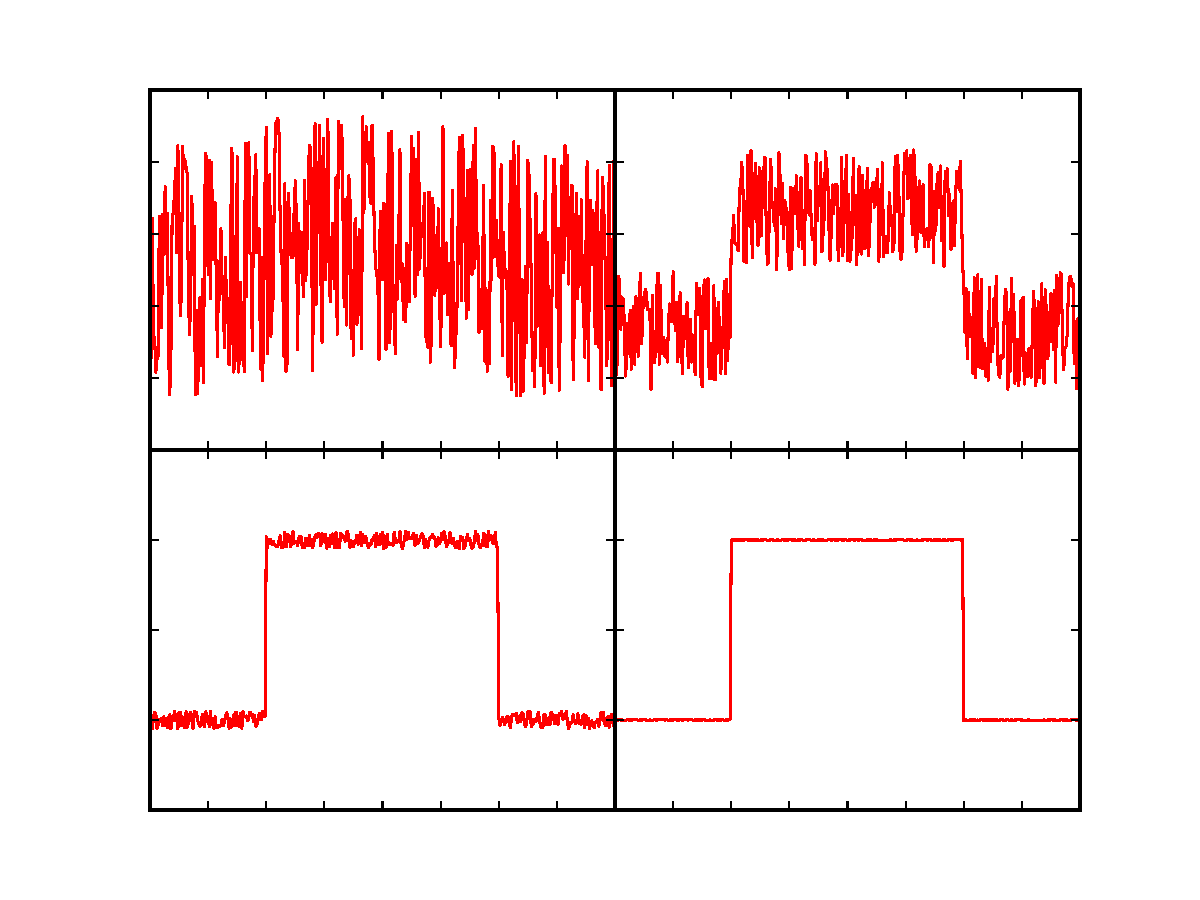
\includegraphics[width = 0.95\textwidth]{figures/SNR_Example}
\caption[Examples of the physical effects of various signal-to-noise ratios]{The effect of increasing the signal-to-noise ratio of a measurement. Left to right, top to bottom: $\mathit{SNR} = 0.1$, $1$, $10$, $100$.}
\label{fig:SNR_example}
\end{center}
\end{figure}
\par 
The physical issues associated with a low signal-to-noise ratio are illustrated in Figure~\ref{fig:SNR_example}. It is clear that, with $\mathit{SNR} = 0.1$ (upper-left in Figure~\ref{fig:SNR_example}), the signal can barely be seen and neither the width nor the amplitude can be ascertained. When the signal-to-noise ratio is increased to unity (upper right in Figure~\ref{fig:SNR_example}), the presence of a signal is clear but there are still significant uncertainties in both the amplitude and the width of the signal. When the signal-to-noise ratio is increased to $10$, these uncertainties are greatly reduced and the pulse can be well characterised. Finally, if the ratio is increased further to $100$, the fluctuations are reduced to such a level that, except under close examination, they are not noticeable.
\par 
The units of noise-equivalent power are $\mathrm{W\,Hz}^{\nicefrac{-1}{2}}$. In order to calculate the noise-equivalent power in the presence of noise sources, such as Johnson noise, which are most commonly measured or calculated as a voltage, these quantities need to be converted into units of Watts. This is done by dividing the noise voltage (units: $\mathrm{V\,Hz}^{\nicefrac{-1}{2}}$) by the voltage responsivity (Equation~\ref{res:Vresponsivity}, units: $\mathrm{V\,W}^{-1}$). Should the noise be measured or calculated in units of amperes (as is the case for Equations~\ref{eqn:NmodNoiseCurrent} and \ref{eqn:NmodPInoise_Golubev}), then the noise needs to be divided by the differential of the $I$-$V$ ($\nicefrac{\partial I}{\partial V}$, units $\mathrm{A\,V}^{-1}$), as well as the responsivity.\footnote{This paragraph assumes the detector is being current biased. Should the biasing signal be a voltage, then sources measured in amperes do not need to be divided by the differential, whereas those measured in volts need to be divided by $\nicefrac{\partial V}{\partial I}$ and the current responsivity is used.}
\par 
The \gls{acr:NEP} is given by the total noise, $e_{\mathrm{tot}}$ divided by the responsivity (i.e. the incident power that would produce a signal equal in amplitude to the noise). This means it can be written as:
\begin{align}
\mathit{NEP} &= \frac{e_{\mathrm{tot}}}{S_{\mathrm{V}}}\,. \label{def:NEP}
\end{align}
\par 
The simplest example of calculating the noise-equivalent power is to take the case where the measured noise is dominated by a single source. In the real world, this is most commonly the case when the amplifier noise in the readout is not low enough. If we take the case where the amplifier noise, $\left<\delta V\right>_{\mathrm{amp}}$, is very large, i.e.:
\begin{align}
\left<\delta V\right>_{\mathrm{amp}} &= 100~\mathrm{nV\,Hz}^{\nicefrac{-1}{2}}\,. 
	\label{eqn:NEPex_largeAmpNoise}
\intertext{Provided that this is significantly larger than any other noise source which contaminates the measurement then:}
e_{\mathrm{tot}} &\approx \left<\delta V\right>_{\mathrm{amp}} \,. 
	\label{eqn:NEpex_AmpNoise_limit}
\intertext{If, in this example, the voltage responsivity was $10^{6}~\mathrm{V\,W}^{-1}$, then the noise-equivalent power would be:}
\mathit{NEP} &= \frac{\left<\delta V\right>_{\mathrm{amp}}}
	{S_{\mathrm{V}}}\,, \\
\mathit{NEP} &= \frac{100 \times 10^{-9}}{10^{6}}\,, \\
\mathit{NEP} &= 1 \times 10^{-13}~\mathrm{W\,Hz}^{\nicefrac{-1}{2}}\,. 
	\label{eqn:NEPex_end}
\end{align}
\par 
In order to arrive at a term for the total noise-equivalent power of a detector system which includes a non-perfect amplifier, the various noise terms need to be converted into noise-equivalent powers and then added.
\par 
Taking the noise terms individually, it is possible to see the specific conversions needed to change them to units of $\mathit{NEP}$ ($\mathrm{W\,Hz}^{\nicefrac{-1}{2}}$).
\par 
For a voltage amplifier (as was always used for the experiments in this thesis), the noise is in units of $\mathrm{V\,Hz}^{\nicefrac{-1}{2}}$ so division by the responsivity (which converts between volts and watts) is the only required step to convert the amplifier noise into a noise-equivalent power. 
\begin{align}
\mathit{NEP}_{\mathrm{amp}} = & \frac{\left<\delta V\right>_{\mathrm{amp}}}{S_{\mathrm{V}}}\,. \label{eqn:NEP_amp}
\end{align}
\par 
A brief inspection of the units of the heat-flow noise ($\left<\delta P\right>$) shows that this term, as expected, is already a noise-equivalent power:
\begin{align}
\left<\delta P\right> &= \sqrt{2EP_{\mathrm{N}}}\,, 
	\tag{\ref{eqn:Nmod_GolubevPnoise} revisited} \\
&= \sqrt{\mathrm{J\,W}}\,, \label{eqn:PnoiseUnits} \\
&= \sqrt{\mathrm{Ws\,W}} \,, \\
&= \sqrt{\mathrm{W^{2}s}} \,, \\
&= \sqrt{\mathrm{W^{2}\,Hz^{-1}}}\,, \\
\therefore \quad \left<\delta P\right> &= \mathrm{W\,Hz}^{\nicefrac{-1}{2}}\,,\\
\therefore \quad \mathit{NEP}_{\mathrm{P}}&= \left<\delta P\right>\,. \label{eqn:NEP_P}
\end{align} 
\par 
A similar treatment reveals that the electron-phonon heat-flow noise ($\left<\delta P\right>_{\mathrm{e\mbox{-}ph}}$) is also already in units of noise-equivalent power:
\begin{align}
\left<\delta P\right>_{\mathrm{e\mbox{-}ph}} &= \sqrt{2\beta k_{\mathrm{B}}\varSigma\varOmega
	\left(T_{\mathrm{e}}^{\beta+1} + T_{\mathrm{ph}}^{\beta+1}\right)}\,, 
	\tag{\ref{eqn:e-phNoise} revisited} \\
&= \sqrt{\mathrm{J\,K^{-1}\, W\,K}^{-\beta}\,\mathrm{m^{-3}
	\,m^{3}\,K}^{\beta+1}}
	\,, \label{eqn:e-phNoiseUnits} \\
&= \sqrt{\mathrm{J\,W}}\,, 
\end{align}
which is the same as Equation~\ref{eqn:PnoiseUnits}. Therefore:
\begin{align}
\left<\delta P\right>_{\mathrm{e\mbox{-}ph}} &= \mathrm{W\,Hz}^{\nicefrac{-1}{2}}\,, \\
\therefore \quad \mathit{NEP}_{\mathrm{e\mbox{-}ph}} &= \left<\delta P\right>_{\mathrm{e\mbox{-}ph}} \,. 
	\label{eqn:NEP_e-ph}
\end{align}
\par 
By dimensional analysis, the units of the tunnelling current noise are shown to be $\mathrm{A\,Hz}^{\nicefrac{-1}{2}}$:
\begin{align}
\left<\delta I\right> &= \sqrt{2eI}\,, \tag{\ref{eqn:SchottkyNoise} revisited}\\
&= \sqrt{\mathrm{C\,A}}\,, \\
&= \sqrt{\mathrm{As\,A}}\,, \\
\therefore \quad &= \mathrm{A\,Hz}^{\nicefrac{-1}{2}}\,. 
	\label{eqn:currentNoiseUnits} \\
\intertext{This means that the tunnelling shot noise-equivalent power, $\mathit{NEP}_{\mathrm{S}}$, can be found by dividing the current shot noise by both the differential of the current by the voltage and voltage responsivity, i.e.:}
\mathit{NEP}_{\mathrm{S}} &= \frac{\sqrt{2eI}}{\frac{\partial I}{\partial V} S_{\mathrm{V}}} \,. 
	\label{eqn:NEP_shot}
\end{align}
\par 
The final noise term to inspect is the correlator of the noise due to the tunnelling power and current ($\left<\delta P \delta I\right>$). This is found to have units of $\mathrm{AW\,Hz}^{-1}$:
\begin{align}
\left<\delta P \delta I\right> &= -4eP\,, 
	\tag{\ref{eqn:NmodPInoise_Golubev} revisited} \\
&= \mathrm{C\,W}\,, \\
&= \mathrm{As\,W}\,, \\
\therefore \quad \left<\delta P \delta I\right> &= \mathrm{AW\,Hz}^{-1}\,, 
	\label{eqn:PInoise_units}
\intertext{which makes sense considering that, dimensionally, this is just the multiplication of $\left<\delta P\right>$ and $\left<\delta I\right>$. This means that the noise-equivalent power due to this correlation of terms, $\mathit{NEP}_{\mathrm{PI}}$, is given by:}
\mathit{NEP}_{\mathrm{PI}} &= 2C\sqrt{\frac{eP}{\frac{\partial I}{\partial V}S_{\mathrm{V}}}}\,, \\
\mathit{NEP}_{\mathrm{PI}} &= -2\sqrt{\frac{eP}{\frac{\partial I}{\partial V}S_{\mathrm{V}}}}
	\label{eqn:NEP_PI}
\end{align} 
\par 
Having converted the various noise sources into units of $\mathit{NEP}$, it is possible to arrive at a final equation for the total noise-equivalent power of a cold-electron bolometer, $\mathit{NEP}_{\mathrm{CEB}}$. This is found by simply adding the uncorrelated noise terms in quadrature, with the addition of the cross-correlator of the power and current shot noise. This gives the final result for a current-biased device (i.e. a system using a voltage readout) to be:
\begin{align}
\mathit{NEP}_{\mathrm{CEB}}^{2} = \frac{\left<\delta V^{2}\right>_{\mathrm{amp}}}{S_{\mathrm{V}}^{2}}
	&+ 2\beta k_{\mathrm{B}}\varSigma\varOmega
		\left(T_{\mathrm{e}}^{\beta+1} + T_{\mathrm{ph}}^{\beta+1}\right)\nonumber \\
	&+ \left<\delta P^{2}\right> 
	-2 \frac{\left<\delta P \delta I\right>}{\frac{\partial I}{\partial V}S_{\mathrm{V}}}
	+ \frac{\left<\delta I^{2}\right>}
		{\left(\frac{\partial I}{\partial V}S_{\mathrm{V}}\right)^{2}}\,,
	\label{res:NEP_CEB}
\end{align}
It is not advisable to write this equation more thoroughly (as was done for Equations~\ref{res:CurrentNoise} and \ref{res:powerNoise}) as this would be several pages long.
%
\subsection{Photon Noise}\label{ssec:photonNoise}
In addition to the internal noise sources of the detector and those associated with the readout circuitry, there is another (often limiting) source which it is important to consider. This is the noise associated with the absorption of photons at the detectors. There are two main terms which combine here and these are the photon shot noise and the photon wave noise. The origins of these two terms come from the particle and wave models of light, respectively. At high frequencies, where light is often thought of as distinct particles, it is clear that there should be no correlation between the arrival of one photon and the arrival of the next, but instead, the arrival of photons is governed by Poisson statistics. The noise-equivalent power associated with this model of light is given by the well-known equation:
\begin{align}
\mathit{NEP}_{\mathrm{ph_{shot}}}^{2} = 2h\nu P_{\mathrm{opt}}\,,
	\label{eqn:photonShotNoise}
\end{align}
where $\nu$ is the frequency of the light and $P_{\mathrm{opt}}$ is the optical power absorbed by the detector. However, at lower frequencies, such a model of light is not valid and instead, one must think of light as a wave. Clearly, in such a scenario, the arrival of one maximum at the detector heavily determines the arrival of the next---they are highly correlated. Simplistically, what was previously thought of a single photon is now represented by a wave \textit{packet}. These wave packets interfere with one another, causing fluctuations in the power arriving at the detector. This leads to the photon wave noise-equivalent power, which is given by the, also well known, equation:
\begin{align}
\mathit{NEP}^{2}_{\mathrm{ph_{wave}}} 
	= \frac{P^{2}_{\mathrm{opt}}}{\Delta\nu}\,,
	\label{eqn:photonWaveNoise}
\end{align}
where $\Delta\nu$ is the optical bandwidth. For black-body emission, two regimes exist; these are the Wien region (sometimes called the Wien tail, where $h\nu \gg k_{\mathrm{B}}T$) and the Rayleigh-Jeans region (where $h\nu \ll k_{\mathrm{B}}T$). In the first of these, the photon model is more appropriate and the first term (Equation~\ref{eqn:photonShotNoise}) dominates. However, in the Rayleigh-Jeans region, a wave-type model of light is more appropriate and, as such, the second term (Equation~\ref{eqn:photonWaveNoise}) dominates. However, the most complete treatment may be found by considering both of these terms together and, as such, the total photon noise-equivalent power is given by:
\begin{align}
\mathit{NEP}_{\mathrm{ph}}^{2} = 2h\nu P_{\mathrm{opt}} + \frac{P_{\mathrm{opt}}^{2}}{\Delta \nu}\,.
	\label{eqn:photonNoise}
\end{align}
